\documentclass[journal]{IEEEtran}
\usepackage[T1]{fontenc}
\usepackage[utf8]{inputenc}
\usepackage{amsmath,amssymb,amsfonts}
\usepackage{graphicx}
\usepackage{booktabs}
\usepackage{multirow}
% siunitx removed: the only usage was an unused \sisetup call (no \SI/\si/
% \num/\ang commands appear anywhere in the body), and the siunitx.sty
% available for this compile (v2.1l, 2011) predates the modern expl3/LaTeX3
% kernel installed here, causing a hard compile failure on load. Reinstate
% with a current siunitx (v3.x) if unit-formatting commands are added later.
\usepackage{xcolor}
\usepackage{url}
\usepackage{cite}
\usepackage{algorithm}
\usepackage{algpseudocode}
\usepackage{balance}
\usepackage{xspace}

\graphicspath{{figures/}}

\newcommand{\healpix}{HEALPix\xspace}
\newcommand{\dggs}{DGGS\xspace}
\newcommand{\utm}{UTM\xspace}
\newcommand{\psf}{PSF\xspace}
\newcommand{\R}{\mathbb{R}\,}
\newcommand{\Nside}{N_{\mathrm{side}}\,}
\newcommand{\mgrs}{\textsc{mgrs}}
\newcommand{\argmin}{\mathop{\mathrm{arg\,min}}\,}

\begin{document}

\title{\texttt{healpix-resample}: PSF-Aware Resampling of Earth-Observation Imagery onto HEALPix}

\author{
Jean-Marc Delouis\textsuperscript{1},
Tina Odaka\textsuperscript{1},
Benoit Bovy\textsuperscript{2},
Etienne Cap\textsuperscript{1},
Thomas Davison\textsuperscript{6},
Anne Fouilloux\textsuperscript{3},
Camille Gueguen\textsuperscript{1},
Alexander Kmoch\textsuperscript{4},
Justus Magin\textsuperscript{1},
Pablo Richard\textsuperscript{5},
and Vincent Dumoulin\textsuperscript{6}%
\thanks{\textsuperscript{1}LOPS UMR 6523,
CNRS--IFREMER--IRD--Univ. Brest--IUEM, Plouzané, France.
Corresponding author: jean.marc.delouis@ifremer.fr.}%
\thanks{\textsuperscript{2}GEORODE, Liège, Belgium.
Email: bbovy@georode.com.}%
\thanks{\textsuperscript{3}LifeWatch ERIC, Seville, Spain.
Email: anne.fouilloux@lifewatch.eu.}%
\thanks{\textsuperscript{4}University of Tartu,
Institute of Ecology and Earth Sciences,
Landscape Geoinformatics Lab, Tartu, Estonia.
Email: alexander.kmoch@ut.ee.}%
\thanks{\textsuperscript{5}Pablo Richard EI, Paris, France.
Email: pablorichard@hotmail.fr.}%
\thanks{\textsuperscript{6}European Space Agency (ESA)---ESRIN, Frascati, Italy.
Email: vincent.dumoulin@esa.int.}%
}

\markboth{IEEE Journal of Selected Topics in Applied Earth Observations and Remote Sensing}%
{Delouis \MakeLowercase{\textit{et al.}}: PSF-Aware HEALPix Resampling for Earth Observation}

\maketitle

\begin{abstract}
Earth-observation products are commonly distributed on local projected grids,
whereas global and multi-sensor analyses increasingly use hierarchical
spherical grids such as \healpix. Their conversion is not purely geometric:
each measured pixel represents a spatially integrated observation of an
underlying field.

We introduce \texttt{healpix-resample}, a \psf-aware framework that jointly
models the sensor response and the source-to-\healpix geometry. Its two
dual-normalized transfer operators form an exact adjoint pair under
grid-dependent weighted inner products, yielding a sparse weighted
least-squares problem solved without explicit matrix inversion. This
reformulation turns resampling into GPU-tractable map-making and provides a
basis for future fusion in which heterogeneous observations constrain one
latent \healpix field while retaining their own spatial responses. In controlled
synthetic-detector experiments, the matched model gives the lowest RMSE against
the known pre-degradation reference in all four scene types and recovers 17--22\% of
the error introduced by the prescribed blur. A geographically distributed
validation over 40 independent regions and 358 valid patches confirms this
result: region-cluster bootstrap intervals are positive in every scene class,
with mean recovery of 15.4--19.6\%, and the matched reconstruction has lower
RMSE than all five multi-region comparators on every valid patch. In a
separate one-patch-per-region ablation, joint inversion also outperforms
both Richardson--Lucy and Tikhonov deconvolution followed by geometric
regridding in all 40 regions. A real-radiometry control with an imposed
$24\times45$~m anisotropic response, reconstructed with the current
isotropic model, retains the same ranking across all four scenes.

On Sentinel-2 B04 imagery, the \utm--\healpix--\utm round trip reaches RMSE
between $2.8\times10^{-6}$ and $1.0\times10^{-5}$, demonstrating numerical
consistency with the input rather than independent recovery of the instrumental
\psf. A downscaling experiment addresses this limitation: against a reference
independent of the imposed 20~m degradation, the matched method has the lowest
RMSE in all 38 real Sentinel-2 regions tested, against each of four
competitors (exact sign test $p=7.3\times10^{-12}$; mean paired margins
$10.3$--$17.9\%$ over the strongest of them). A four-scene version of the same
test ranks it first under an estimator-independent geometric control and under
an anisotropic $24\times45$~m degradation, and its ranking survives a
$\pm20\%$ error in the assumed response width -- the level the spectral
calibration leaves unresolved. Spectral
diagnostics support stable partial restoration, while noise experiments show
that the preferred damping depends on noise amplitude and covariance. On an
NVIDIA A100 GPU, median operator-construction-plus-solve time is $0.32$~s per
$256\times256$ patch over 357 timed patches.
\end{abstract}

\begin{IEEEkeywords}
Discrete Global Grid Systems, DGGS, HEALPix, Sentinel-2, point spread function, resampling, regridding, inverse problems, Earth observation, UTM.
\end{IEEEkeywords}

\section{Introduction}
\label{sec:introduction}

Earth-observation (EO) products are made available in a broad range of local map projections, tiling schemes, and sensor-dependent sampling geometries. Sentinel-2 Level-2A data, for instance, are delivered as ortho-images on the \utm/WGS84 grid, with ground sampling distances of 10, 20, or 60~m, depending on the spectral band
\cite{esa_sentinel2_handbook,copernicus_sentinel2_l2a}. While such projected products are convenient for regional-scale processing, they make global, multi-resolution, and multi-sensor analyses more difficult.

Discrete Global Grid Systems (DGGS) offer an alternative representation by dividing the Earth into hierarchically organized, globally indexed cells \cite{ogc_dggs_2021,Kmoch2022}. Within this family, \healpix provides equal-area cells, hierarchical indexing, and iso-latitude sampling, which makes it well suited for global EO data cube applications \cite{gorski2005healpix}. Nevertheless, the discrete resolution levels of a DGGS typically do not match the native sampling of a given sensor. In the experiments discussed here, a Sentinel-2 band with a 10~m sampling interval is mapped onto a level-20 \healpix grid whose cell widths are about 6.22~m. Inferring values on this finer grid is thus more than a simple coordinate transformation: it entails identifying which spatial details are genuinely supported by the available observations.

Traditional resampling techniques---such as nearest-neighbor, bilinear, and cubic interpolation---tackle this issue from a purely geometric perspective. They estimate target pixel values from neighboring source samples based on their spatial coordinates, without explicitly accounting for how the measurements themselves were generated \cite{esa_snap_resampling,gdal_resampling,schowengerdt_resampling}. In reality, each recorded pixel corresponds to the underlying continuous field convolved with a finite spatial response that encompasses optical blur, detector integration, platform motion, atmospheric influences, and prior processing. This spatial response is typically characterized by a point spread function (\psf) or a modulation transfer function. Neglecting it during resampling can lead to extra smoothing and alter the spatial power spectrum of the resulting data \cite{inamdar2023sr2,schowengerdt2007remote,kaur2024spatial}.

When the target grid has a finer resolution than the original sampling, PSF-aware resampling becomes closely connected to image restoration and model-based super-resolution. The goal is not to fabricate independent sub-pixel details, but to infer a latent field whose spatial response is still compatible with the acquired image. This inverse problem is only partially constrained---especially at higher spatial frequencies---and thus demands explicit regulation of the poorly observed components \cite{richardson1972bayesian,lucy1974iterative,elad1997restoration,park2003superresolution,farsiu2004advances}.

We present \texttt{healpix-resample}, a \psf-aware framework
for transferring projected EO images onto \healpix
(Fig.~\ref{fig:workflow}). Pixels on
the source grid are interpreted as sparse, spatially weighted
samples of an underlying \healpix field. Two dual-normalized
transfer operators connect the source and target grids, forming
an exact adjoint pair with respect to grid-dependent weighted
inner products. The latent field is estimated via a matrix-free,
weighted inverse problem that simultaneously accounts for the
assumed spatial response and the combined projected-grid--\healpix
geometry. The approach is sensor-agnostic and relies only on
sample geolocations and an effective spatial-response model.

The validation addresses three complementary questions. First, a
controlled synthetic-detector experiment uses Esri World
Imagery as a high-resolution spatial texture, convolves it with
a known Gaussian \psf, and compares the reconstructed field with
the original pre-degradation reference
\cite{esri_world_imagery}. This experiment evaluates spatial
restoration and enables direct comparison with geometric
interpolation, Richardson--Lucy deconvolution followed by
regridding, and deliberately mis-specified \psf models. Second,
a real Sentinel-2
\utm--\healpix--\utm experiment evaluates whether the inferred
\healpix field retains the information required to reproduce the
original projected-grid observation. This round trip measures
numerical consistency with the input data; it is not presented
as independent validation of the true instrumental \psf. Third, a
real-data downscaling experiment (Section~\ref{sec:real_downscale_experiment})
degrades real, undegraded Sentinel-2 pixels to a coarser grid and
    compares the reconstruction against a reference constructed independently
    of the imposed degradation from the same real imagery, thereby
providing a reconstruction-quality assessment on real data without
relying on the Esri texture as a Sentinel-2 radiometric proxy. It is run
over 38 geographically distributed regions drawn from the same site list as
the synthetic validation, so the two share their sampling of the globe.

The use of a \healpix support finer than the native sensor grid
may increase the number of stored values. This cost must
ultimately be compared with the overlap and duplicated coverage
already present in projected tiling systems such as Sentinel-2
UTM/MGRS \cite{bauer2023wasting}. Storage, compression,
chunking, and multi-resolution encoding are not addressed here
and will be examined in a dedicated study.

The main contributions of this work are:

\begin{itemize}
    \item a sparse \psf-aware observation model that replaces direct
    geometric resampling by a model-consistent inverse problem on
    \healpix, made computationally practical by sparse GPU operators;

    \item a formulation in which multiple acquisitions or detectors,
    each with its own sampling geometry and spatial response, can in
    principle constrain a shared latent field;

    \item a dual-normalized weighted-adjoint formulation and a
    matrix-free iterative solver whose per-iteration cost scales
    linearly with the number of source samples for a fixed
    neighborhood size;

    \item a controlled synthetic-detector validation over urban,
    water, forest, and agricultural scenes, including a 40-region
    replication, spectral diagnostics, \psf-mismatch experiments,
    and comparison with geometric, Richardson--Lucy, and Tikhonov
    baselines;

    \item a real Sentinel-2 round-trip experiment that evaluates
    compatibility between the reconstructed \healpix field and
    the original projected-grid observation;

    \item a real-data downscaling experiment that evaluates
    reconstruction quality on real Sentinel-2 imagery against a reference
    independent of the imposed degradation, over 38 geographically
    distributed regions, complemented by an estimator-independent geometric
    control and an anisotropic response-shape mismatch control;

    \item an open-source implementation designed for
    \healpix/DGGS-based EO data-cube workflows
    \cite{healpix_resample_repo}.
\end{itemize}

An optional extension for exact conservation of area-integrated
quantities is presented separately in
Appendix~\ref{app:conservative}.

\section{Background and Related Work}

\subsection{HEALPix as a Latent Spherical Support}

The \healpix tessellation divides the sphere into $12\Nside^2$ equal-area cells, with $\Nside=2^L$ at hierarchy level $L$ \cite{gorski2005healpix,calabretta2007healpix}. Its equal-area, hierarchical, and iso-latitude properties make it useful for area-consistent statistics, multi-resolution indexing, and efficient spherical data access.

Here \healpix serves as a latent spherical support rather than a sensor-specific sampling grid; the method depends on neither a particular sensor resolution nor a fixed level. Sentinel-2 imagery is only a representative high-resolution optical test case, for which we take $L=20$ ($\Nside=1{,}048{,}576$, cell size $\approx6.22$~m). This makes the target support finer than the native 10~m sampling, but the same formulation applies to coarser or finer sensors and other DGGS resolutions.

When the target grid is finer than the native sampling, the problem has more degrees of freedom than observations, so the finer grid does not by construction carry independent information at the target-cell scale. Those extra degrees of freedom must instead be constrained by the forward observation model, the effective spatial response, and regularization, as in image restoration and super-resolution.

\healpix is supported by a mature software ecosystem: the
reference \texttt{healpy} library provides pixelization and
spherical-harmonic transforms \cite{zonca2019healpy}, and
\texttt{cdshealpix-python} efficient indexing and geometric
operations \cite{cdshealpix2021}. For Earth observation, the
GRID4EARTH project develops a complementary stack of
\texttt{healpix-geo}, \texttt{healpix-resample},
\texttt{healpix-analyse}, and \texttt{healpix-plot}, distributed
through the \texttt{grid4earth} meta-package
\cite{grid4earth_tools}. The present implementation belongs to
that stack and uses \texttt{healpix-geo} rather than
\texttt{healpy} for indexing, coordinate conversion, cell
geometry, and neighbourhood calculations
\cite{healpix_geo_repo,healpix_resample_repo}. \texttt{healpix-geo}
(Apache-2.0) supports both the conventional spherical geometry and
an ellipsoidal formulation in which geodetic coordinates on a
reference ellipsoid such as WGS84 are mapped onto an authalic
sphere before indexing, preserving equal area on the ellipsoidal
Earth \cite{healpix_geo_repo}; the sparse transfer operators can
therefore be built consistently under either convention.

General-purpose EO resampling toolkits such as
\texttt{pyresample} already offer nearest-neighbour and
Gaussian-weighted regridding onto \healpix and other target grids
\cite{hoese2020pyresample}, but do not pose the target-grid values
as the solution of an inverse observation problem with an explicit
sensor \psf. The proposed method is thus complementary to the
existing \healpix and EO ecosystems, while relying on the
GRID4EARTH geometry layer for ellipsoid-aware coordinates.

\psf-aware resampling has also been addressed outside the DGGS
context. The SR2 workflow \cite{inamdar2023sr2} explicitly
incorporates a sensor spatial response when resampling
hyperspectral imagery, but in the opposite direction to the
present work: it \emph{degrades} a high-resolution raster to
simulate the coarser spatial response of a target sensor, so
that hyperspectral data can be realistically compared against or
substituted for coarser-resolution imagery. The problem addressed
here is the inverse one -- recovering a latent field at a finer,
DGGS-indexed resolution from a coarser, \psf-blurred observation
-- posed as a regularized inverse problem with an explicit
adjoint pair of transfer operators, rather than as a forward
degradation model. The two approaches share the premise that
ignoring the sensor spatial response during resampling is a
methodological error, but target opposite ends of the same
resampling operation.

\subsection{Resampling as an Observation Model}

In this work, resampling is formulated as an observation model rather than as a purely geometric interpolation. The projected image is treated as a set of spatially weighted measurements of a latent \healpix field, with weights determined by geolocation and by an assumed effective \psf. This connects the method to classical inverse formulations used in deconvolution, super-resolution, and model-based image reconstruction \cite{bertero1998inverse,starck1998deconvolution,richardson1972bayesian,lucy1974iterative,park2003superresolution}.

The scientific motivation for this change is to preserve the relationship between the reconstructed field and the measurement process; GPU execution is an enabling technology rather than the justification for the model. Sparse operators and matrix-free iterations make an inverse formulation affordable at the scale of routine patch processing, as quantified in Section~\ref{sec:hpx_datacube_implications}. This viewpoint also connects resampling to map-making methods in which redundant observations constrain a common map and, when the model is sufficiently identifiable, instrumental nuisance parameters. For example, SRoll2 fits higher-order instrumental-response parameters from Planck data redundancy while constructing frequency maps~\cite{delouis2019sroll2}. The present work makes no equivalent calibration claim: geolocation and the effective \psf are held fixed, and only the latent spatial field is estimated.

The objective is not blind super-resolution from a single image, but controlled inverse resampling: the recovered \healpix field is explicitly tied to the assumed observation operator and constrained by regularization.

Framed this way, the observation model makes very few structural assumptions about its input: each source sample contributes a value, a geolocation, and an assumed local spatial response, with no requirement that the samples originate from a single regular raster or a single acquisition. Section~\ref{sec:outlook_fusion} returns to this point and outlines how the mathematical formulation extends by stacking observation blocks for multiple overlapping acquisitions and for sensors whose measurements are not grid-aligned. The released implementation does not yet expose all of this generality.

\section{Method}

\subsection{Dual-Normalized Transfer Operators}
\label{sec:dual_normalized_operators}

Let $\mathbf{y}\in\mathbb{R}^{N}$ denote the vectorized image
patch on the projected source grid, where $N$ is the number of
valid source pixels. Let $\mathbf{x}\in\mathbb{R}^{M}$ denote a
field defined on the $M$ retained \healpix cells covering the
image patch.

The implementation uses two sparse transfer operators with
complementary normalization conventions. The first operator maps
a \healpix field to the source observation grid, whereas the
second maps source-grid values to an initial \healpix estimate.
The two operators use the same spatial neighbourhoods and the
same unnormalized Gaussian weights, but they are not exact
transposes of one another.

For source pixel $i$ and retained \healpix cell $j$, let
$d_{ij}$ denote their local geodesic distance. The unnormalized
spatial weight is

\begin{equation}
g_{ij}
=
\exp\left(
-\frac{2d_{ij}^{2}}{s_{\psf}^{2}}
\right),
\label{eq:raw_weight}
\end{equation}

where $s_{\psf}$ controls the width of the effective spatial
response. With this convention, the corresponding full width at
half maximum is

\begin{equation}
\mathrm{FWHM}
=
\sqrt{2\ln 2}\,s_{\psf}.
\label{eq:fwhm_code}
\end{equation}

To maintain sparsity, each source pixel is connected only to a
fixed number $q$ of nearby retained \healpix cells. In addition,
candidate cells whose accumulated Gaussian influence remains
below a prescribed threshold are excluded from the reconstructed
support.

We define the forward observation operator
$\mathbf{A}\in\mathbb{R}^{N\times M}$ by normalizing the weights
independently for each source pixel:

\begin{equation}
A_{ij}
=
\frac{g_{ij}}
{\displaystyle
 \sum_{k\in\mathcal{N}(i)}g_{ik}},
\qquad
j\in\mathcal{N}(i),
\label{eq:forward_operator}
\end{equation}

where $\mathcal{N}(i)$ is the set of retained \healpix neighbours
associated with source pixel $i$. This normalization gives

\begin{equation}
\sum_{j\in\mathcal{N}(i)} A_{ij}=1,
\end{equation}

so that the source-grid prediction

\begin{equation}
\widehat{\mathbf{y}}
=
\mathbf{A}\mathbf{x}
\label{eq:forward_prediction}
\end{equation}

preserves a spatially constant \healpix field.

A second operator
$\mathbf{B}\in\mathbb{R}^{M\times N}$ is constructed by
normalizing the same raw weights independently for each retained
\healpix cell, optionally scaled by a per-source-pixel area (or
more generally, weight) $a_i\geq0$:

\begin{equation}
B_{ji}
=
\frac{g_{ij}\,a_i}
{\displaystyle
 \sum_{\ell:\,j\in\mathcal{N}(\ell)}g_{\ell j}\,a_\ell},
\qquad
j\in\mathcal{N}(i).
\label{eq:back_operator}
\end{equation}

For every retained cell -- i.e.\ every cell whose accumulated influence passed the support threshold above, so that at least one source sample contributes to it --

\begin{equation}
\sum_{i:\,j\in\mathcal{N}(i)}B_{ji}=1.
\end{equation}

$\mathbf B$ thus performs a normalized, area-weighted local averaging of source-grid values onto the \healpix lattice: a source pixel spanning a larger physical area contributes proportionally more to a given cell, rather than every pixel contributing equally regardless of size. This mitigates biases from varying source-pixel area but does not by itself conserve a globally area-integrated quantity. Setting $a_i\equiv1$ recovers the area-agnostic normalization. The forward operator $\mathbf A$ is left unweighted: \healpix cells are equal-area by design, and---as shown below---$a_i$ cancels analytically from $\mathbf A$'s per-source-pixel normalization anyway.

If $a_i$ is not supplied, the implementation estimates exact
spherical-zone areas for regular latitude rings, including reduced
Gaussian grids. Projected or scattered grids fall back to
$a_i\equiv1$; users requiring area weighting for such grids must
supply it explicitly.

Because the source pixels and \healpix cells have different
sampling geometries and different normalization requirements,
the two operators generally satisfy

\begin{equation}
\mathbf{B}\neq\mathbf{A}^{\mathsf T}.
\label{eq:not_adjoint}
\end{equation}

Both operators derive from the same area-weighted raw weight
$g'_{ij}:=g_{ij}a_i$. The factor $a_i$ cancels from each row of
$\mathbf A$ but remains in the column normalization of $\mathbf B$.
Introduce the corresponding diagonal normalizers

\begin{equation}
\begin{split}
\mathbf{D}_y&=\operatorname{diag}\!\left(d^{A}_i\right),\;\;
d^{A}_i=\sum_{k\in\mathcal N(i)}g_{ik}\,a_i,\\
\mathbf{D}_x&=\operatorname{diag}\!\left(d^{B}_j\right),\;\;
d^{B}_j=\!\!\sum_{\ell:\,j\in\mathcal N(\ell)}\!\!g_{\ell j}\,a_\ell,
\end{split}
\label{eq:dxdy}
\end{equation}

where $\mathbf D_y$ acts on source samples and $\mathbf D_x$ on
retained \healpix cells. Direct substitution gives

\begin{equation}
\mathbf{B}=\mathbf{D}_x^{-1}\mathbf{A}^{\mathsf T}\mathbf{D}_y.
\label{eq:weighted_adjoint}
\end{equation}

Thus $\mathbf B$ is the exact adjoint of $\mathbf A$ under the
weighted inner products
$\langle\mathbf u,\mathbf v\rangle_{\mathbf D_x}
=\mathbf u^{\mathsf T}\mathbf D_x\mathbf v$ on the \healpix support
and
$\langle\mathbf p,\mathbf q\rangle_{\mathbf D_y}
=\mathbf p^{\mathsf T}\mathbf D_y\mathbf q$ on the source grid. The
method is therefore a weighted least-squares formulation with an
exact non-Euclidean operator--adjoint pair.

\subsection{Reference Estimate and Damped Residual Correction}

The source-to-\healpix operator is first used to construct a
reference estimate

\begin{equation}
\mathbf{x}_{\mathrm{ref}}
=
\mathbf{B}\mathbf{y}.
\label{eq:xref}
\end{equation}

This field is a locally normalized weighted average of the source
observations on the retained \healpix cells. Applying the forward
operator gives the source-grid prediction associated with this
initial estimate,

\begin{equation}
\mathbf{y}_{\mathrm{ref}}
=
\mathbf{A}\mathbf{x}_{\mathrm{ref}}.
\end{equation}

The method then estimates a correction
$\boldsymbol{\delta}\in\mathbb{R}^{M}$ from the source-grid
residual

\begin{equation}
\mathbf{r}_{\mathrm{ref}}
=
\mathbf{y}
-
\mathbf{A}\mathbf{x}_{\mathrm{ref}}.
\label{eq:initial_residual}
\end{equation}

The correction is defined by the damped linear system

\begin{equation}
\left(
\mathbf{B}\mathbf{A}
+
\lambda\mathbf{I}
\right)
\boldsymbol{\delta}
=
\mathbf{B}
\left(
\mathbf{y}
-
\mathbf{A}\mathbf{x}_{\mathrm{ref}}
\right),
\label{eq:correction_system}
\end{equation}

where $\lambda\geq0$ controls the magnitude of the correction.
The final reconstructed field is

\begin{equation}
\widehat{\mathbf{x}}
=
\mathbf{x}_{\mathrm{ref}}
+
\boldsymbol{\delta}.
\label{eq:final_estimate}
\end{equation}

The damping term plays the role of a Tikhonov-style
regularizer~\cite{tikhonov1977solutions}, but acts on the
correction relative to the initial normalized estimate, rather
than directly penalizing the norm of the final field. Increasing $\lambda$ keeps the solution closer
to $\mathbf{x}_{\mathrm{ref}}$, whereas a smaller value allows a
larger correction of the residual spatial response. Consequently,
$\lambda$ controls both the amplification of measurement
perturbations and the bias retained from the initial estimate; its
useful range depends on the noise covariance and on how strongly
the requested target-grid modes are constrained by the
observations.

Since $\mathbf{B}$ is not the Euclidean transpose of
$\mathbf{A}$, Eq.~\eqref{eq:correction_system} is not the normal
equation of the Euclidean Tikhonov problem
$\|\mathbf{A}\mathbf{x}-\mathbf{y}\|_2^2+\lambda\|\mathbf{x}\|_2^2$.
Using the weighted-adjoint relation of
Eq.~\eqref{eq:weighted_adjoint}, it is instead exactly the
stationarity condition of the weighted damped least-squares
problem

\begin{equation}
\begin{split}
\widehat{\boldsymbol\delta}
=
\arg\min_{\boldsymbol\delta}\;
\left\|\mathbf A\boldsymbol\delta-\mathbf r_{\mathrm{ref}}\right\|^2_{\mathbf D_y}
+
\lambda\left\|\boldsymbol\delta\right\|^2_{\mathbf D_x},
\\
\|\mathbf z\|^2_{\mathbf D}:=\mathbf z^{\mathsf T}\mathbf D\mathbf z,
\end{split}
\label{eq:weighted_variational}
\end{equation}

with $\mathbf r_{\mathrm{ref}}$ defined in Eq.~\eqref{eq:initial_residual}. Setting the gradient of Eq.~\eqref{eq:weighted_variational} to zero yields $\mathbf A^{\mathsf T}\mathbf D_y(\mathbf A\boldsymbol\delta-\mathbf r_{\mathrm{ref}}) +\lambda\mathbf D_x\boldsymbol\delta=\mathbf 0$. Left-multiplying by $\mathbf D_x^{-1}$ and inserting Eq.~\eqref{eq:weighted_adjoint} leads exactly back to Eq.~\eqref{eq:correction_system}. For $\lambda=0$, the system becomes positive semi-definite, and the solution may no longer be unique if the target field includes more degrees of freedom than there are observations. In the numerical experiments, CG is started from the zero vector and terminated after at most 14 iterations, which selects a particular Krylov-subspace solution and yields an implicit iterative regularization.

\subsection{Matrix-Free Iterative Solution}
\label{sec:matrix_free_solution}

The current implementation solves
Eq.~\eqref{eq:correction_system} using a matrix-free
conjugate-gradient iteration~\cite{hestenes1952cg}; a matrix-free LSQR
iteration~\cite{paige1982lsqr} would apply equally to the same weighted
normal equations and is not explored here. The composite matrix
$\mathbf{B}\mathbf{A}$ is never assembled explicitly. For a trial
correction $\mathbf{v}$, the required operator application is
evaluated as

\begin{equation}
\mathbf{v}
\mapsto
\mathbf{B}
\left(
\mathbf{A}\mathbf{v}
\right)
+
\lambda\mathbf{v}.
\label{eq:matrix_free_operator}
\end{equation}

Each iteration therefore requires one sparse application of
$\mathbf{A}$ and one sparse application of $\mathbf{B}$. If each
source pixel is connected to at most $q$ retained \healpix cells,
then both operators contain at most approximately $qN$ non-zero
coefficients. The resulting per-iteration computational cost is

\begin{equation}
\mathcal{O}
\left(
\operatorname{nnz}(\mathbf{A})
+
\operatorname{nnz}(\mathbf{B})
\right)
=
\mathcal{O}(qN).
\end{equation}

For a fixed neighbourhood size $q$, the per-iteration cost
therefore scales linearly with the number of source pixels. The
total cost is

\begin{equation}
\mathcal{O}(n_{\mathrm{it}}qN),
\end{equation}

where $n_{\mathrm{it}}$ is the number of iterations performed.

Because the two transfer operators are independently normalized,
the composite operator $\mathbf H=\mathbf B\mathbf A+\lambda\mathbf I$
is not Euclidean-symmetric. It is, however, self-adjoint and
positive-definite in the $\mathbf D_x$-weighted inner product: by
Eq.~\eqref{eq:weighted_adjoint},
$\mathbf D_x\mathbf H=\mathbf A^{\mathsf T}\mathbf D_y\mathbf A+\lambda\mathbf D_x$,
symmetric positive-definite in the Euclidean sense for
$\lambda>0$ (semi-definite for $\lambda=0$). Conjugate gradients
therefore remains justified, provided its own inner products use
that weighted metric: every dot product
$\langle\mathbf u,\mathbf v\rangle$ in the standard recursion
becomes $\langle\mathbf u,\mathbf v\rangle_{\mathbf D_x}
=\mathbf u^{\mathsf T}\mathbf D_x\mathbf v
=\sum_j d^{B}_j\,u_jv_j$, with $d^{B}_j$ the per-cell weights of
Eq.~\eqref{eq:dxdy} (\texttt{cell\_weight} in the released code).
Standard CG theory therefore applies only when the recursion uses
the $\mathbf D_x$ metric. A Euclidean-inner-product implementation
has no such guarantee; on synthetic systems built from the same
weights it produced slower and less regular residual reduction.
This observation is empirical, not a monotonicity theorem.
Convergence is monitored through the $\mathbf D_x$-weighted
residual norm.

The correction minimizes a weighted residual but does not enforce
conservation of an area-integrated quantity. Appendix~\ref{app:conservative}
evaluates two optional conservative extensions on ERA5 flux data;
neither is used in the Sentinel-2 experiments.

\subsection{Round-Trip Prediction}

After reconstruction, the inferred \healpix field is projected
back onto the source grid using the forward operator:

\begin{equation}
\widehat{\mathbf{y}}
=
\mathbf{A}\widehat{\mathbf{x}}.
\label{eq:roundtrip_prediction}
\end{equation}

The round-trip residual is

\begin{equation}
\mathbf{r}
=
\widehat{\mathbf{y}}
-
\mathbf{y}.
\label{eq:roundtrip_residual}
\end{equation}

This residual measures compatibility between the reconstructed
\healpix representation and the original source-grid observation
under the dual-normalized transfer model. It does not constitute
an independent validation of the assumed spatial response or of
an unknown unblurred radiance field.


\begin{algorithm}[t]
\caption{Dual-normalized \psf-aware projected-grid--\healpix
resampling.}
\label{alg:psf_resampling}
\begin{algorithmic}[1]
\Require Source image $\mathbf{y}$, source geolocation,
\healpix level $L$, Gaussian scale $s_{\psf}$,
neighbour count $q$, support threshold, damping parameter
$\lambda$, optional per-pixel area $\mathbf a$
\Ensure Reconstructed \healpix field $\widehat{\mathbf{x}}$
and optional source-grid prediction $\widehat{\mathbf{y}}$

\State Identify candidate \healpix cells around the source
image patch.
\State Compute raw Gaussian weights
$g_{ij}=\exp(-2d_{ij}^{2}/s_{\psf}^{2})$.
\State Retain cells whose accumulated influence exceeds the
support threshold.
\State Associate each source pixel with its $q$ nearest retained
\healpix cells.
\State Construct the source-prediction operator $\mathbf{A}$ by
normalizing weights over the \healpix neighbours of each source
pixel.
\State Construct the source-to-\healpix aggregation operator
$\mathbf{B}$ by normalizing weights over the source pixels
contributing to each \healpix cell, scaled by $\mathbf a$ if
supplied (auto-estimated from shared-latitude rings otherwise,
else uniform).
\State Compute the reference field
$\mathbf{x}_{\mathrm{ref}}=\mathbf{B}\mathbf{y}$.
\State Solve
\[
(\mathbf{B}\mathbf{A}+\lambda\mathbf{I})
\boldsymbol{\delta}
=
\mathbf{B}
(\mathbf{y}-\mathbf{A}\mathbf{x}_{\mathrm{ref}})
\]
using the matrix-free iterative solver, with CG inner products
evaluated in the $\mathbf D_x$-weighted metric of
Eq.~\eqref{eq:dxdy}.
\State Set
$\widehat{\mathbf{x}}
=\mathbf{x}_{\mathrm{ref}}+\boldsymbol{\delta}$.
\State Optionally compute
$\widehat{\mathbf{y}}=\mathbf{A}\widehat{\mathbf{x}}$.
\Comment{An optional exact-conservation variant of this step is
given in Appendix~\ref{app:conservative}.}
\end{algorithmic}
\end{algorithm}

\begin{figure*}[t]
\centering

\includegraphics[width=0.95\linewidth]{figures/fig01_psf_healpix_workflow.pdf}
\caption{PSF-aware projected-grid--HEALPix resampling workflow. The projected source image is modeled as a sparse set of spatially weighted measurements of a latent \healpix field. The recovered field can be stored directly in a DGGS representation or mapped back to the source grid to evaluate consistency with the original observation space.}
\label{fig:workflow}
\end{figure*}

\section{Validation Strategy}
\label{sec:validation}
\subsection{Overview}
\begin{figure*}[t]
\centering
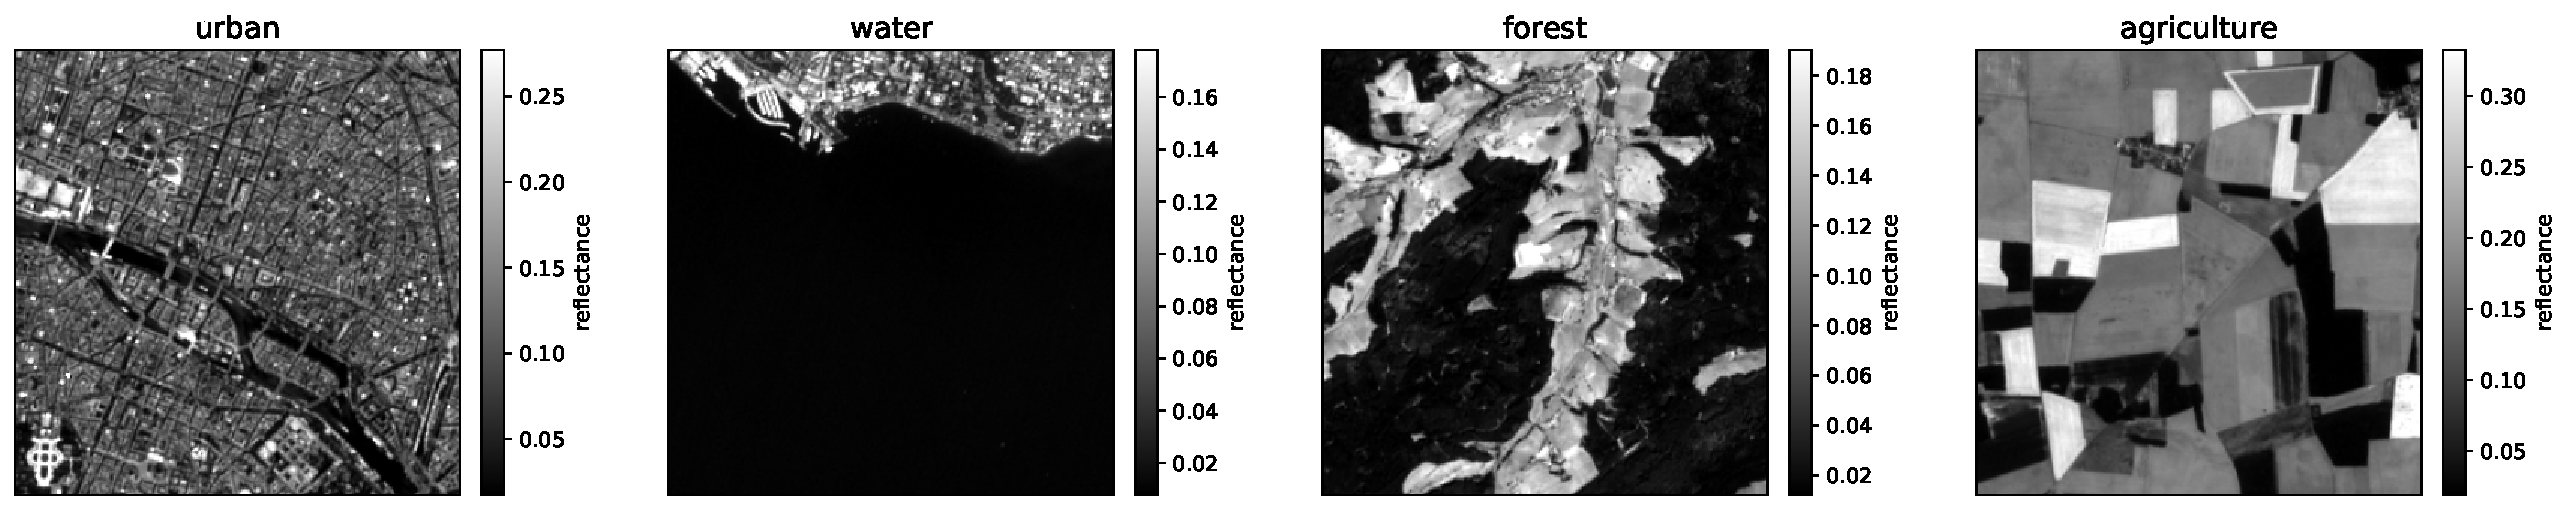
\includegraphics[width=\textwidth]{scene_types.pdf}
\caption{Representative image patches for the four scene types used in the validation experiments: urban, water, forest, and agriculture. The scenes cover contrasting spatial structures, including dense linear features, homogeneous surfaces, irregular natural textures, and piecewise homogeneous fields with sharp boundaries. Each panel uses an independent reflectance scale.}
\label{fig:validation_scenes}
\end{figure*}
The validation uses four contrasting scene types: urban, water,
forest, and agriculture, shown in
Fig.~\ref{fig:validation_scenes}. Three complementary experiments
are considered. A controlled synthetic-detector experiment
evaluates recovery relative to a known pre-degradation texture, a real
Sentinel-2 round trip evaluates whether the reconstructed
\healpix field remains compatible with the original projected-grid
observation, and a real-data downscaling experiment evaluates
reconstruction quality against a reference constructed independently
of the imposed degradation from real, undegraded imagery. The
round trip is a consistency test and cannot by itself validate
recovery of an unknown unblurred scene; the real-data downscaling
experiment is designed to close that gap without depending on the
Esri texture as a proxy for Sentinel-2 radiometry.

In all recovery experiments, every method is evaluated on the same
\healpix cell-average estimand. For the geometric baselines, the
interpolated raster is sampled at the level-22 child-cell centres and
the 16 samples are averaged within each level-20 parent cell. The
round-trip readout uses the corresponding interpolation order on the
source grid. Exact conservation of area-integrated quantities is
treated separately in Appendix~\ref{app:conservative}.

\subsection{Controlled Synthetic Detector Experiment}
\label{sec:controlled_synthetic}

For each scene, an Esri World Imagery patch is used as a
high-resolution spatial texture rather than as a Sentinel-2
radiometric reference \cite{esri_world_imagery}. The texture is
blurred using a prescribed Gaussian response and sampled onto a
synthetic 10~m detector grid. The resulting observation is
resampled onto \healpix, and the reconstructed field is compared
with both the original texture and its blurred counterpart.

This experiment separates the latent texture, the detector
response, and the reconstructed grid representation. It therefore
evaluates whether the inversion partially restores attenuated
spatial information when the target \healpix support is finer
than the simulated detector sampling.


\subsection{Real Projected-Grid Round-Trip Experiment}
\label{sec:roundtrip_experiment}

The second experiment uses Sentinel-2 patches over the same four
scene types. Because no unblurred reference is available, it does
not constitute an absolute deconvolution benchmark. Instead, it
tests whether the estimated \healpix field preserves the
information required to predict the original source-grid
observation.

Let $\mathbf{y}$ denote the input image,
$\widehat{\mathbf{x}}$ the reconstructed \healpix field, and
$\widehat{\mathbf{y}}=\mathbf{A}\widehat{\mathbf{x}}$ its
source-grid prediction. The round-trip residual is

\begin{equation}
\mathbf{r}
=
\widehat{\mathbf{y}}-\mathbf{y}.
\label{eq:residual}
\end{equation}

A small residual indicates consistency with the input observation
under the assumed operator; it does not demonstrate that the true
instrumental \psf has been inverted.


\subsection{Real-Data Downscaling Experiment}
\label{sec:real_downscale_experiment}

The controlled synthetic-detector experiment
(Section~\ref{sec:controlled_synthetic}) validates spatial
restoration against a known reference, but that reference is an
Esri World Imagery texture rather than Sentinel-2 radiometry, and
the same prescribed \psf both generates and inverts the synthetic
observation. The round trip
(Section~\ref{sec:roundtrip_experiment}) uses real Sentinel-2 data
but cannot by itself demonstrate recovery of an unknown unblurred
scene (Section~\ref{sec:roundtrip_interpretation}). This third
experiment partly addresses that gap, evaluating reconstruction quality on
real Sentinel-2 pixels against a reference built independently of
the degradation under test but not independently of the estimator family.

For each scene, the real native 10~m B04 patch serves two separate
roles. First, as the best available estimate of the true field: the
undegraded pixels are resampled with the matched \psf-aware
operator onto a level-20 \healpix grid, using the same
$\mathrm{FWHM}=12.5$~m response and configuration as
Section~\ref{sec:exp_config}, and the result is downgraded to
level 19 (cell size $\approx12.44$~m) by a plain unweighted average
of each cell's level-20 children -- a purely geometric aggregation
with no spatial-response model. This level-19 field is the
reference for every method below; built entirely from step 2, it
depends only on the real, undegraded imagery, not on any subsequent
blurring or reconstruction.

Second, and independently, the same native 10~m patch is
Gaussian-blurred to $\mathrm{FWHM}=25$~m -- $1.25\times$ the
target 20~m sampling, so that the response still matters at the
target grid -- and point-sampled every other pixel to give a
synthetic 20~m observation. Decimation rather than block-averaging
is deliberate: averaging a $2\times2$ block on top of an
already-blurred field adds a boxcar (square, non-circular)
component to the true degradation kernel, which the isotropic
Gaussian weights of Eq.~\eqref{eq:experimental_gaussian} cannot
represent. Decimating keeps the true degradation kernel exactly the shape the
inverse model assumes, so that any difference between methods is attributable
to the reconstruction rather than to a shape the test introduced. The
anisotropic control below shows this precaution is not the decisive one --
the method tolerates a far more severe shape error -- but it costs nothing and
removes the question from the primary comparison. The 20~m samples are then resampled
onto the reference's level-19 grid using the matched $25$~m
response, and every method under test -- \psf-aware,
nearest-neighbor, bilinear, bicubic, and Richardson--Lucy
deconvolution followed by bicubic interpolation -- is evaluated at
exactly the same cell centers, restricted to cells at least
$8\times25=200$~m inside the patch interior. The protocol mirrors
the controlled synthetic experiment (blur, sample, resample,
compare) but uses real Sentinel-2 data throughout, and separates
reference construction from the degradation-and-reconstruction
pipeline under test.

As a response-shape mismatch control, we repeat the degradation with a
strongly anisotropic Gaussian in the projected-grid axes,
$\mathrm{FWHM}_x=24$~m and $\mathrm{FWHM}_y=45$~m. The current
\texttt{PSFResampler} interface and the Richardson--Lucy comparator both
retain the scalar isotropic $25$~m response during reconstruction. This
deliberately unmatched experiment therefore measures robustness to an
unmodelled response shape; it is not an implementation test of an
anisotropic inverse kernel. To limit boundary contamination, evaluation
is restricted to cells at least $8\times45=360$~m inside the patch.

\subsubsection{Geographic Extension of the Downscaling Experiment}
\label{sec:real_downscale_multiregion}

Four scenes make a case study, not a population. We therefore repeat the
identical seven-step protocol at the \emph{same 40 region anchors} used by
the synthetic multi-region validation of Section~\ref{sec:multiregion}, one
patch per region, so that the real and synthetic experiments sample the same
sites and the region remains the independent statistical unit.

These patches are real Sentinel-2 acquisitions, not the Esri textures of the
synthetic experiment, with which they share only the site list. They are read
as Cloud-Optimized GeoTIFFs from the Element~84 \texttt{earth-search}
catalogue \cite{earthsearch}, which holds the complete Sentinel-2 L2A archive;
the EOPF Zarr Sample Service catalogue used for the four scenes of
Section~\ref{sec:exp_config} (\texttt{stac.core.eopf.eodc.eu}) is a regional
demonstration service and returns no product at most of these anchors. Products are selected deterministically
by lowest cloud cover, and the resulting product identifier is recorded with
each patch.

Two screens then decide which regions enter the analysis, both reading only
the observation. The first rejects a patch whose window is clipped at a
granule edge, carries no-data holes, is flat, or is covered by cloud or snow
despite a low granule-level cloud fraction; all 40 patches pass it. The
second requires a region to evaluate at least half the median number of
interior \healpix cells: one region yields no evaluable cells and another only
$448$ of a typical $29{,}900$, both because reference and reconstruction
barely overlap after the edge margin. Retaining them would let a region scored
on $1.5\%$ of its area carry the same weight in a region-level mean as a
complete one.

Thirty-eight regions remain -- eight agricultural and ten of each other class
-- contributing $29{,}795$--$29{,}955$ interior cells each. The evaluated-cell
count is identical across all five methods within a region, since they are
scored on the same cells, so neither screen can select for or against a
reconstruction method.

\subsection{Experimental Configuration}
\label{sec:exp_config}

All experiments use $256\times256$ patches. The real-data evaluation uses the Sentinel-2 Level-2A red band (B04) on its native 10~m \utm grid, about $2.56\times2.56$~km per patch, selected with a maximum cloud cover of $20\%$; missing pixels are filled with the patch mean of the valid pixels. Throughout, the effective instrumental response is $\mathrm{FWHM}=12.5~\mathrm{m}$, i.e.\ a Gaussian scale $s_{\mathrm{op}}=s_{\mathrm{gen}}=10.62\,\mathrm{m}$ through Eq.~\eqref{eq:fwhm_code}. Section~\ref{sec:psf_calibration} shows the resulting synthetic spectra reproduce the observed B04 slopes in all four scenes, and the value is independently bracketed by the ESA MSI MTF-at-Nyquist specification. It is therefore an empirically supported effective B04 response, not a claimed unique optical-PSF measurement.

The target support is a nested \healpix grid at level $L=20$,
with $N_{\mathrm{side}}=2^{20}$ and an equivalent cell size of
approximately $6.22$~m. Each source sample is associated with
its $q$ nearest retained \healpix cells, where $q$ is chosen so
that at least $99\%$ of the kernel's weight is retained given
$s_{\mathrm{op}}$ and the level-20 cell size ($q=22$ for the
matched configuration), and cells whose accumulated Gaussian
weight remains below $0.1$ are excluded. The matched
reconstruction uses conjugate gradients with a light damping of
$\lambda=10^{-3}$, at most 14 iterations, and a relative residual
tolerance of $10^{-8}$. This fixed value is used as a controlled
default for the main comparison and is not presented as a
noise-adaptive optimum.

For the synthetic experiment, Esri imagery is sampled at Web
Mercator zoom level 17, converted to grayscale luminance, and
evaluated on a grid oversampled by a factor of four relative to
the 10~m detector grid. The high-resolution texture is convolved
with an isotropic Gaussian kernel using reflective boundary
conditions and then averaged over $4\times4$ blocks. No
additional measurement noise is introduced in the primary synthetic
comparison; Section~\ref{sec:noise_robustness} reports a separate
noise-injection experiment using the same four scenes.

Both the synthetic detector and the matched inverse operator use
the Gaussian width parameter

\begin{equation}
s_{\mathrm{op}}=s_{\mathrm{gen}}=10.62~\mathrm{m},
\end{equation}

with weights defined by

\begin{equation}
w(d)
=
\exp\left(
-\frac{2d^2}{s_{\mathrm{op}}^2}
\right).
\label{eq:experimental_gaussian}
\end{equation}


\subsubsection{PSF-Mismatch Sensitivity Test}
\label{sec:psf_mismatch}

Sensitivity to spatial-response uncertainty is evaluated by
repeating the reconstruction with

\begin{equation}
s_{\mathrm{op}}=15.92~\mathrm{m}\quad(q=48)
\end{equation}

for the \emph{PSF-aware $+50\%$} case and

\begin{equation}
s_{\mathrm{op}}=5.31~\mathrm{m}\quad(q=9)
\end{equation}

for the \emph{PSF-aware $-50\%$} case -- i.e.\ $\mathrm{FWHM}=18.75~\mathrm{m}$ and $\mathrm{FWHM}=6.25~\mathrm{m}$ respectively. A common damping of $\lambda=10^{-3}$ is used for the matched and both mismatched configurations in all four scenes. This keeps the sensitivity test attributable to the assumed response width rather than to arm-specific regularization.

We also use Richardson--Lucy deconvolution \cite{richardson1972bayesian,lucy1974iterative} as a conventional two-stage baseline: deconvolution on the \utm grid with the generation \psf, then transfer to \healpix by bicubic upsampling to an intermediate $5~\mathrm{m}$ grid and averaging over the level-22 children of each level-20 cell -- the same cell-average estimand as every other method in Table~\ref{tab:synthetic_metrics} (Section~\ref{sec:estimand}). An earlier version instead took a single bilinear point sample at each cell centre, which put Richardson--Lucy at an avoidable disadvantage unrelated to the deconvolution itself, and was replaced by the matching cell-average procedure.

Concretely, the baseline uses \texttt{skimage.restoration.richardson\_lucy}: the synthetic \utm data are rescaled to $[0,1]$ and deconvolved for 100 fixed iterations (no adaptive stopping) with the matched Gaussian response used to generate them, converted to $\sigma=\mathrm{FWHM}/(2\sqrt{2\ln2})$ in source-pixel units and truncated at $4\sigma$. The result is computed with \texttt{clip=False}, returned to the original radiometric scale, then upsampled and rebinned as above, mirroring how the cell-average reference values are built.

The Tikhonov baseline introduced in Section~\ref{sec:rl_ablation} uses the
closed-form Fourier filter $\widehat x=H^*\widehat y/(|H|^2+\lambda_{\mathrm{Tik}})$
with $\lambda_{\mathrm{Tik}}=10^{-2}$ and the same matched Gaussian response;
the FFT implementation implies circular boundary conditions. Neither this
parameter nor the 100-iteration Richardson--Lucy stopping point was tuned per
scene. Their comparison is therefore a fixed-configuration ablation, not an
optimized ranking of deconvolution algorithms.

Reference values on the level-20 \healpix grid are obtained by
sampling the high-resolution texture at the centers of its 16
nested level-22 child cells and averaging the samples. The same
procedure is applied to the blurred texture.

For the spectral analysis, each image is independently normalized
between its first and ninety-ninth percentiles, clipped to
$[0,1]$, and mean-centered. A two-dimensional Hann window is
applied before Fourier transformation, and the reported
one-dimensional spectra are obtained by azimuthally averaging the
squared Fourier amplitudes.

\subsection{Empirical Consistency Check of the Effective B04 Spatial Response}
\label{sec:psf_calibration}

The effective Gaussian $\mathrm{FWHM}=12.5~\mathrm{m}$ used
throughout this paper (Section~\ref{sec:exp_config}) is selected
from a direct comparison with real Sentinel-2 B04 spectra rather
than from any single synthetic scene. The resulting synthetic
power-spectrum slopes are checked independently against the
isotropically averaged spectra of all four real B04 patches.

\begin{figure*}[t]
\centering
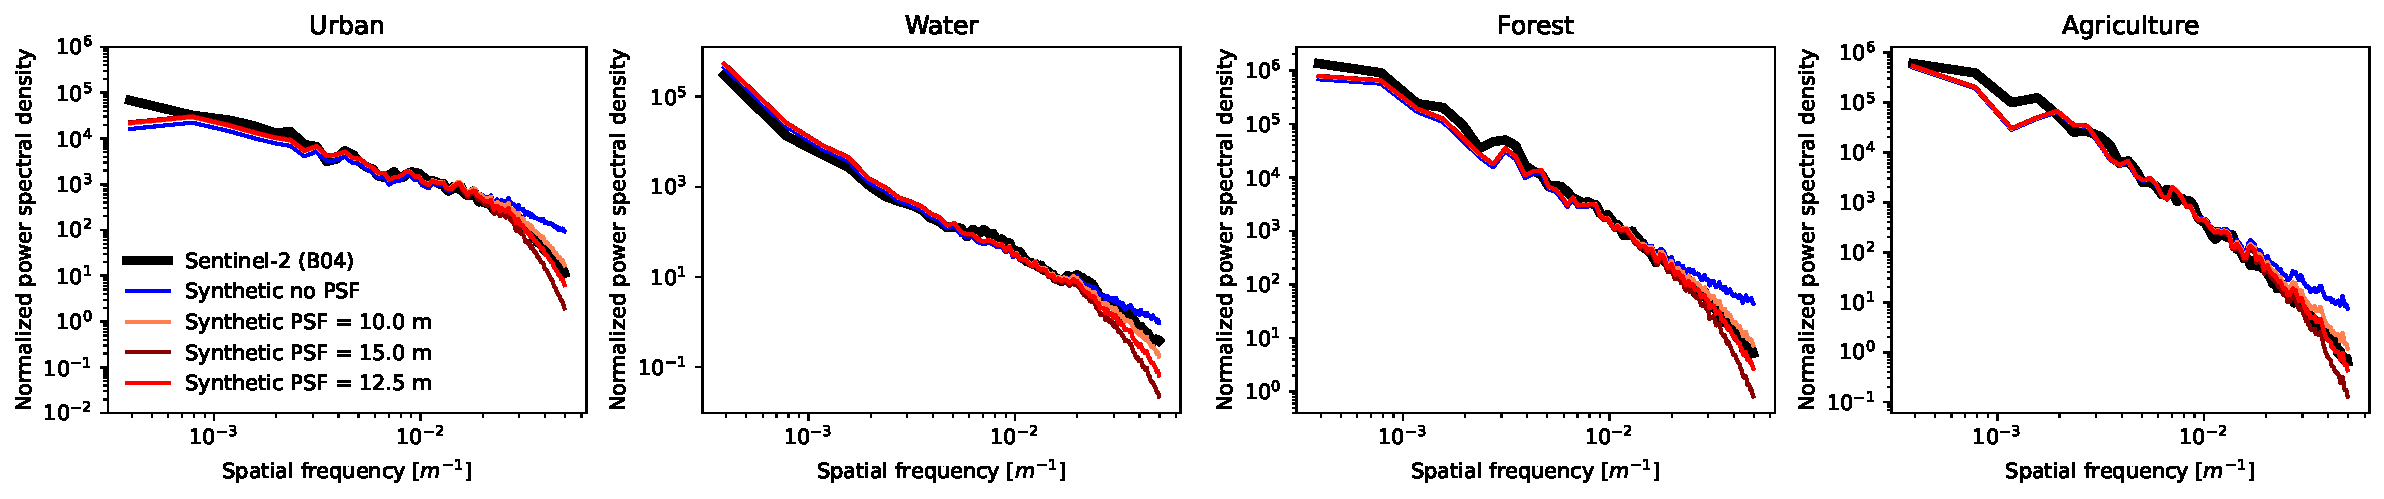
\includegraphics[width=\textwidth]{figures/synthetic_vs_sentinel2.pdf}
\caption{Power spectra of real Sentinel-2 B04 patches (black)
compared with the synthetic Esri-latent-texture pipeline of
Section~\ref{sec:controlled_synthetic} blurred at three candidate
Gaussian widths, $\mathrm{FWHM}\in\{10.0,12.5,15.0\}~\mathrm{m}$
($0.8\times$, $1.0\times$, and $1.2\times$ the value used
elsewhere in this paper), for the urban, water, forest, and
agriculture scenes. Each synthetic curve is independently
amplitude-matched to the real spectrum over an intermediate
  frequency band ($0.0039$--$0.0195~\mathrm{m}^{-1}$; radial bins
  10--50 on the $256\times256$, 10~m grid) before comparison, so that only the
spectral \emph{shape} is being compared, not the absolute power
level. The pre-degradation no-\psf synthetic spectrum is shown for
reference (blue). The $12.5$~m curve reproduces the observed B04
spectral slopes across the four scene types over the resolved
comparison range.}
\label{fig:psf_calibration}
\end{figure*}

Figure~\ref{fig:psf_calibration} is an empirical consistency check
of the adopted response scale. After amplitude matching, the
$12.5$~m pipeline reproduces the observed B04 spectral slopes in all
four scenes. The three candidate widths remain close over much of
the resolved range, however, so the comparison does not uniquely
distinguish $12.5$~m from its $\pm20\%$ alternatives.

At high frequency, the real urban, forest, and agricultural spectra
retain more power than any of the noise-free synthetic blurred
curves. This excess is consistent with a measurement-noise floor or
with unmodelled processing and scene-spectrum differences; the
present comparison does not identify these contributions
separately.

The scale is independently corroborated by the official Sentinel-2
MSI characterization. The specified system MTF at Nyquist is
$0.15$--$0.30$ for 10~m and 20~m bands, and the published per-band
PSFs are approximated from MTF measurements using Gaussian
modelling~\cite{esa_s2_mtf_technical_guide}. At the 10~m sampling of
B04, this range corresponds to a Gaussian FWHM of
$11.6$--$14.6$~m; conversely, $12.5$~m gives an MTF of $0.249$ at
Nyquist. Together with the spectral slopes, this supports
$12.5$~m as a plausible effective operating point for the
experiments, not as a unique measurement of the optical or
processed Level-2A response. A dedicated slant-edge or point-target
calibration would be required to separate the natural scene
spectrum, processing response, and measurement noise.

\subsection{Multi-Region Synthetic Validation}
\label{sec:multiregion}

The experiment of Sections~\ref{sec:exp_config}--\ref{sec:psf_mismatch} uses a single illustrative patch per scene class and therefore cannot, by itself, support a statistically powered claim about the method's typical behaviour. We complement it with a larger, geographically distributed validation built on the same synthetic Esri pipeline, \psf-aware operator, and geometric baselines.

For each scene class, ten geographically distinct regions were selected, stratified by class rather than sampled at random over the planet. Each region was split into nine non-overlapping $256\times256$ patches on a deterministic $3\times3$ grid with $4$~km spacing, giving 40 regions and 360 selected patches, of which 358 are analysed (Section~\ref{sec:multiregion_results}). All operator parameters match Sections~\ref{sec:exp_config}--\ref{sec:psf_mismatch}: $\mathrm{FWHM}=12.5$~m, level $L=20$, $q=22/48/9$ for the matched/$+50\%$/$-50\%$ arms, and a common damping $\lambda=10^{-3}$. The multi-region experiment is therefore a geographically distributed replication of the Table~\ref{tab:synthetic_metrics} configuration for the matched and width-mismatch arms.

The patches are not treated as independent observations. The nine patches drawn from a given region are spatially correlated sub-samples, so the independent statistical unit is the region: $n=10$ regions per scene class, $n=40$ regions in total. Confidence intervals use 5000 region-cluster bootstrap replicates (seed 20260818), resampling regions with replacement and averaging patches within each resampled region. With ten regions per class, they quantify variation among the selected regions rather than global EO-class uncertainty. We report the recovery fraction

\begin{equation}
\text{recovery}
=
1-\frac{\mathrm{RMSE}(\text{method},\text{latent})}{\mathrm{RMSE}(\text{blurred},\text{latent})},
\label{eq:recovery_fraction}
\end{equation}

for which a positive value indicates recovery relative to the blurred observation and a negative value indicates a reconstruction worse than the blurred observation itself, together with paired per-patch RMSE differences against every competing method and the corresponding win fraction.

This site selection is not intended to generalize to conditions outside the four benchmark classes; clouds, snow and ice, open ocean, mountainous terrain, coastal regions, and incomplete observations remain out of scope (Section~\ref{sec:generalization}). A descriptive breakdown by absolute latitude band is available but is unbalanced -- several class--band combinations contain a single region -- and is not used here to claim latitude invariance or a statistically significant latitude effect.

\subsection{Metrics}

Image-domain fidelity is assessed using the root mean square error (RMSE) and the structural similarity index (SSIM) \cite{wang2004ssim}. RMSE measures the overall amplitude of the reconstruction error, whereas SSIM provides a complementary assessment of structural agreement. These global metrics do not, however, identify the spatial scales at which information is preserved, attenuated, or amplified.

We therefore also compute isotropically averaged one-dimensional power spectra. For a reference spectrum $P_{\mathrm{ref}}(k)$ and an estimated spectrum $P_{\mathrm{est}}(k)$, we define the absolute spectral residual as
\begin{equation}
D_{\mathrm{PSD}}(k)
=
\left|
P_{\mathrm{est}}(k)-P_{\mathrm{ref}}(k)
\right|,
\label{eq:psd_residual}
\end{equation}
where $k$ denotes spatial frequency. This quantity provides a scale-dependent measure of the discrepancy between the estimated and reference fields.

In the controlled synthetic-detector experiment, $P_{\mathrm{ref}}(k)$ is the spectrum of the no-\psf Esri latent texture, allowing the analysis to quantify recovery of spatial frequencies attenuated by the prescribed response. The spectrum of the \psf-blurred synthetic observation is also shown to distinguish partial restoration from simple reproduction of the blurred input. In the real-data round-trip experiment, fidelity is assessed directly in the image domain by comparing the original projected-grid observation $\mathbf{y}$ with the predicted observation $\widehat{\mathbf{y}}$ using RMSE and SSIM. The distinct metric used for the ERA5 flux-conservation experiment, where fidelity to a spatial reference is not the relevant question, is defined separately in Appendix~\ref{app:conservative}.

\section{Results}

\subsection{Controlled Synthetic Detector Recovery}
\label{sec:synthetic_results}

Table~\ref{tab:synthetic_metrics} reports the RMSE of each
reconstruction relative to both the pre-degradation Esri texture and
the corresponding \psf-blurred observation. The matched
\psf-aware reconstruction is the closest to the pre-degradation
reference for all four scene types. Its RMSE is lower than the
degradation introduced by the prescribed blur by approximately
$17$--$22\%$, showing a modest but systematic partial recovery
of spatial information.

The geometric baselines remain closer to the blurred observation,
particularly for bilinear and bicubic interpolation. This is
expected because they interpolate the already degraded samples
without attempting to compensate for the spatial response. Their
low RMSE relative to the blurred reference therefore reflects
preservation of the input blur rather than recovery of the latent
texture.

The PSF-mismatch experiments show that errors in the assumed
response width affect the reconstruction asymmetrically. Using a
PSF that is too narrow (\emph{PSF-aware $-50\%$}) underestimates
the actual blur and therefore applies an insufficient correction.
The resulting field remains under-restored and gives a higher
aggregate RMSE than the matched reconstruction in every scene.

Conversely, using a PSF that is too wide
(\emph{PSF-aware $+50\%$}) makes the inversion compensate for
more attenuation than is actually present. In the present runs its
aggregate RMSE is substantially larger than both the matched result
and the original blur degradation, consistently making it the more
damaging of the two mismatch cases. This error is accompanied by an
amplification of weakly constrained high-frequency components. The corresponding
noise-like instability is more clearly visible in the spectral
diagnostics of Section~\ref{sec:spectral_behaviour}. A nonzero
damping parameter is therefore used for this configuration to
limit the amplification without changing the common damping across
the three arms.

The Richardson--Lucy baseline uses the correct generation PSF
but performs deconvolution on the \utm grid before a separate
cell-average transfer to \healpix (Section~\ref{sec:exp_config}).
In the tested configuration, it remains less accurate than the
matched \psf-aware reconstruction for all four scenes, even
though it is now evaluated on the same cell-average estimand as
every other method. Section~\ref{sec:rl_ablation} repeats this
comparison against a non-iterative Tikhonov baseline on an
identical basis and finds the same ordering, suggesting that the
remaining gap reflects the two-stage deconvolve-then-regrid
structure itself -- rather than a mismatched estimand -- and that
the proposed method's benefit comes from treating the spatial
response and the target-grid geometry jointly rather than
sequentially.

Overall, the matched \psf-aware method provides the best recovery
of the pre-degradation reference among the evaluated approaches.
Underestimating the PSF width mainly leads to under-correction,
whereas overestimating it can produce high-frequency
amplification and may therefore require stronger damping under
noisy conditions.

\begin{table*}[t]
\centering
\caption{RMSE in the controlled synthetic-detector experiment over
the common \healpix cells. The matched and both width-mismatch
configurations use $\lambda=10^{-3}$; $+50\%$ and $-50\%$ denote
overestimated and underestimated operator widths. \emph{Estimated
vs.\ no-\psf} measures recovery of the pre-degradation Esri texture,
whereas \emph{Estimated vs.\ \psf} measures closeness to the blurred
observation. Richardson--Lucy uses the matched PSF followed by
bicubic upsampling and cell-average regridding. Lower is better;
bold marks the minimum in each row. Low geometric-baseline errors
against \emph{Esri PSF} reflect preservation of the input blur, not
restoration quality.}
\label{tab:synthetic_metrics}
\setlength{\tabcolsep}{4pt}
\begin{tabular}{llrrrrrrr}
\toprule
 &  & PSF-aware & PSF-aware & PSF-aware & Richardson--Lucy & Nearest & Bilinear & Bicubic \\
 &  &  & $+50\%$ & $-50\%$ & &  &  &  \\
Scene & Comparison &  &  &  &  &  &  &  \\
\midrule
\multirow[t]{3}{*}{urban} & Estimated vs. Esri no-PSF & \textbf{0.0684} & 0.1426 & 0.0980 & 0.0822 & 0.1056 & 0.1051 & 0.0960 \\
 & Estimated vs. Esri PSF & 0.0525 & 0.1801 & 0.0311 & 0.0189 & 0.0420 & 0.0244 & \textbf{0.0135} \\
 & Esri PSF vs. Esri no-PSF (degradation) & 0.0859 & - & - & - & - & - & - \\
\cline{1-9}
\multirow[t]{3}{*}{water} & Estimated vs. Esri no-PSF & \textbf{0.0213} & 0.0448 & 0.0316 & 0.0257 & 0.0341 & 0.0336 & 0.0304 \\
 & Estimated vs. Esri PSF & 0.0168 & 0.0576 & 0.0109 & 0.0066 & 0.0146 & 0.0082 & \textbf{0.0044} \\
 & Esri PSF vs. Esri no-PSF (degradation) & 0.0273 & - & - & - & - & - & - \\
\cline{1-9}
\multirow[t]{3}{*}{forest} & Estimated vs. Esri no-PSF & \textbf{0.0242} & 0.0463 & 0.0333 & 0.0284 & 0.0363 & 0.0354 & 0.0326 \\
 & Estimated vs. Esri PSF & 0.0171 & 0.0572 & 0.0105 & 0.0064 & 0.0154 & 0.0080 & \textbf{0.0044} \\
 & Esri PSF vs. Esri no-PSF (degradation) & 0.0294 & - & - & - & - & - & - \\
\cline{1-9}
\multirow[t]{3}{*}{agriculture} & Estimated vs. Esri no-PSF & \textbf{0.0155} & 0.0308 & 0.0224 & 0.0184 & 0.0255 & 0.0238 & 0.0214 \\
 & Estimated vs. Esri PSF & 0.0117 & 0.0392 & 0.0086 & 0.0050 & 0.0134 & 0.0060 & \textbf{0.0030} \\
 & Esri PSF vs. Esri no-PSF (degradation) & 0.0191 & -
 & - & - & - & - & - \\
\cline{1-9}
\bottomrule
\end{tabular}
\end{table*}

\subsection{Multi-Region Validation Results}
\label{sec:multiregion_results}

Table~\ref{tab:multiregion} reports the region-level results of the multi-region validation described in Section~\ref{sec:multiregion} ($\lambda=10^{-3}$ common to all three \psf configurations). In every scene class, the matched \psf-aware reconstruction reduces the RMSE relative to the blurred observation, and the region-cluster bootstrap $95\%$ interval for the recovery fraction is strictly positive: from $15.4\%$ [$13.7$, $17.3$] for forest to $19.6\%$ [$18.2$, $21.0$] for urban scenes. The matched reconstruction also has a lower RMSE than every tested competitor -- nearest, bilinear, bicubic, and both mismatched \psf configurations -- on every patch of every scene class (a $100\%$ pairwise win fraction), and the paired RMSE difference against each competitor has a $95\%$ interval that excludes zero in every class.

Two of the ninety water patches were excluded before analysis. Both fall on homogeneous open water in the Caspian Sea, where the prescribed blur degraded the latent texture by a numerically zero RMSE, leaving the recovery fraction of Eq.~\eqref{eq:recovery_fraction} undefined rather than merely small. The criterion depends only on the reference degradation and is evaluated before any reconstruction, so it cannot select for or against any method; the water class therefore contributes 88 patches, and the totals below are 358 rather than the 360 selected.

Both mismatched \psf configurations have a negative mean recovery fraction in every scene class, i.e.\ a higher RMSE than the blurred observation itself, and the $+50\%$ overestimated width is consistently more damaging than the $-50\%$ underestimated width, consistent with the high-frequency amplification discussed in Section~\ref{sec:synthetic_results}. The geometric baselines (nearest, bilinear, bicubic) also have a negative mean recovery fraction in every class: they interpolate the already-blurred field rather than restoring the latent texture, as in the single-patch experiment of Table~\ref{tab:synthetic_metrics}.

The recovery fraction varies by scene class, from about $15.4\%$ for forest to around $19.6\%$ for agriculture and urban scenes; an unweighted average over all 40 regions gives $17.6\%$, but the per-class breakdown is retained because RMSE scales differ substantially between water and urban scenes. Using the same common $\lambda=10^{-3}$ configuration as Table~\ref{tab:synthetic_metrics}, the geographically distributed experiment directly corroborates the four-scene result: recovery remains modest but systematic, and \psf overestimation remains the most damaging width error.

\begin{table*}[t]
\centering
\caption{Multi-region validation with common damping
$\lambda=10^{-3}$. Intervals are $95\%$ region-cluster bootstrap
intervals over ten regions per class. Win fraction is the share of
patches on which the matched reconstruction has lower RMSE than
bicubic interpolation; Section~\ref{sec:multiregion_results} reports
the remaining paired comparisons.}
\label{tab:multiregion}
\setlength{\tabcolsep}{4pt}
\begin{tabular}{lrrrrrr}
\toprule
Scene & Regions & Patches & RMSE blurred & RMSE matched & Recovery [95\% CI] & Win fraction \\
\midrule
Agriculture & 10 & 90 & 0.0276 & 0.0223 & 19.6\% [18.0, 21.1] & 100\% \\
Forest      & 10 & 90 & 0.0308 & 0.0259 & 15.4\% [13.7, 17.3] & 100\% \\
Urban       & 10 & 90 & 0.0635 & 0.0511 & 19.6\% [18.2, 21.0] & 100\% \\
Water       & 10 & 88 & 0.0135 & 0.0114 & 15.8\% [12.1, 19.3] & 100\% \\
\bottomrule
\end{tabular}
\end{table*}

Figure~\ref{fig:multiregion_spectra} shows the corresponding spectral behaviour. For each region, the nine patch spectra are first averaged; the plotted curves are the median of the ten resulting region-mean spectra, and the shaded bands are the descriptive $2.5$th--$97.5$th percentiles across the ten regions. These bands describe geographic variability between regions, not a pixel-wise confidence interval or a standard error, and with only ten regions the extreme percentiles are close to the interpolated min--max envelope; they are widest at high frequency, reflecting scene-to-scene heterogeneity, and the water panel in particular shows several mid-to-high-frequency peaks that are a genuine feature of the underlying regions rather than a plotting artefact.

\begin{figure*}[t]
\centering
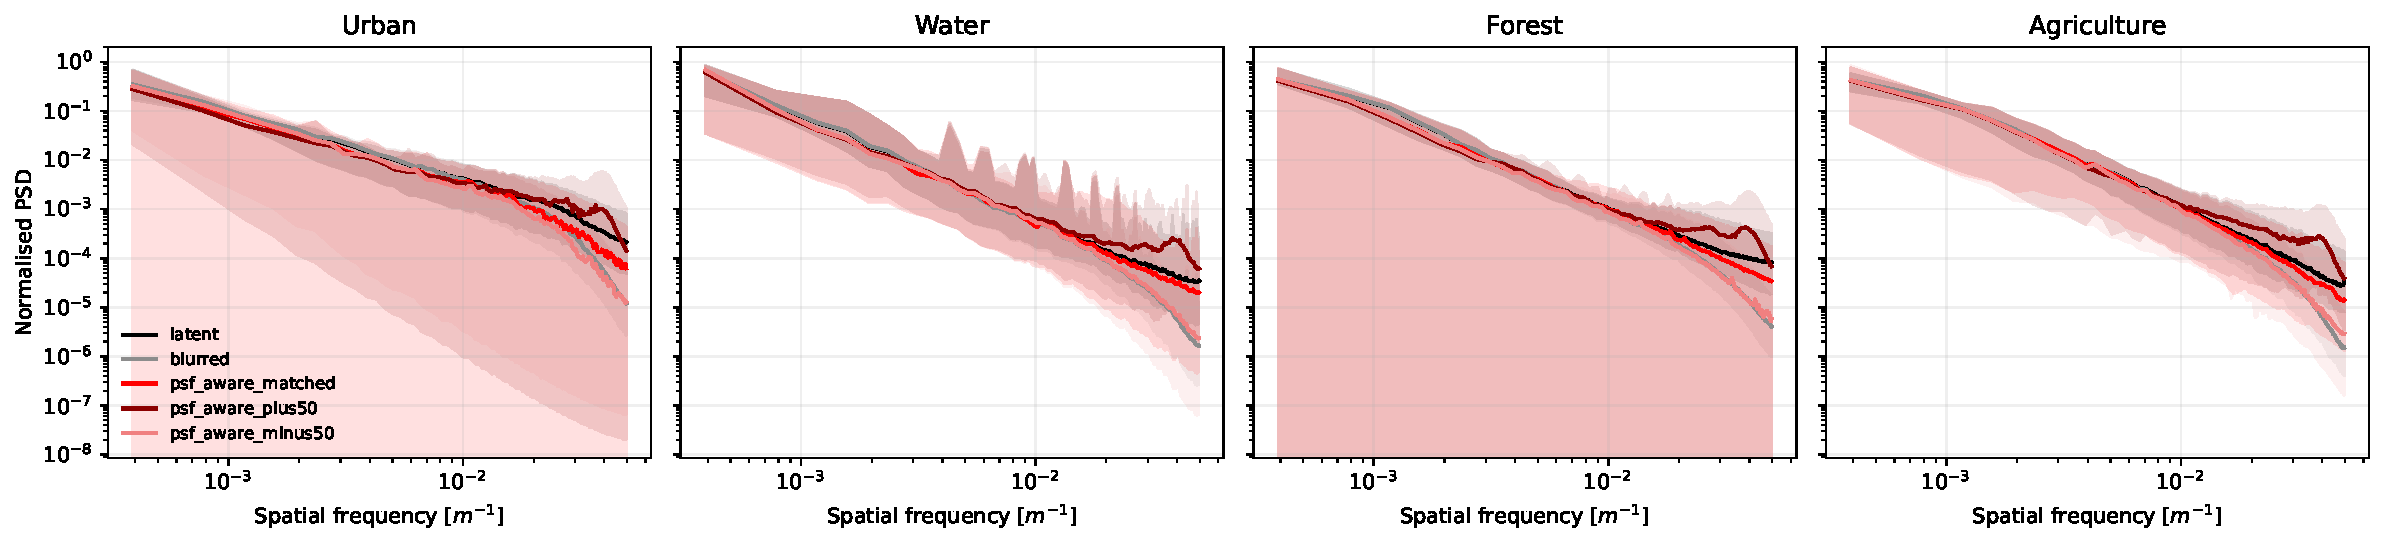
\includegraphics[width=\textwidth]{multi_patch_spectral_uncertainty.pdf}
\caption{Multi-region spectral behaviour for the four scene classes ($\lambda=10^{-3}$ common configuration, Section~\ref{sec:multiregion}). Curves show the median of ten independent region-mean spectra, each itself averaged over nine patches; shaded bands show the descriptive $2.5$th--$97.5$th percentiles across the ten regions, not pixel-wise confidence intervals.}
\label{fig:multiregion_spectra}
\end{figure*}

\subsection{Fair Ablation Against Two-Stage Baselines}
\label{sec:rl_ablation}

The Richardson--Lucy baseline in Table~\ref{tab:synthetic_metrics}
is a two-stage procedure: deconvolution on the \utm grid, followed
by a separate transfer to \healpix. To isolate how much of its gap
to the jointly solved \psf-aware reconstruction is attributable to
the deconvolution step itself, rather than to any residual
estimand mismatch, we compare it with a second, non-iterative
two-stage baseline -- Tikhonov-regularized deconvolution
\cite{tikhonov1977solutions} followed by the identical bicubic
upsampling and cell-average \healpix regridding used for
Richardson--Lucy (Section~\ref{sec:exp_config}) -- and evaluate
both against the pre-degradation no-\psf reference on exactly the same cell-average
basis as the \psf-aware method.

\begin{table*}[t]
\centering
\caption{One-patch-per-region ablation over 40 independent Esri regions
($n=10$ per scene class). The central valid patch is selected using
reference validity before method scores are inspected. All methods are
evaluated against the same pre-degradation, cell-average reference.
$\Delta$ is the paired RMSE difference competitor minus \psf-aware;
positive values favour the proposed method, and brackets give the 95\%
region-bootstrap interval (5000 replicates). The Fourier Tikhonov filter
uses $\lambda_{\mathrm{Tik}}=10^{-2}$ and Richardson--Lucy uses 100 fixed
iterations; neither setting is tuned per region.}
\label{tab:rl_ablation}
\setlength{\tabcolsep}{5pt}
\begin{tabular}{lrrrrr}
\toprule
Scene & PSF-aware & Tikhonov+bicubic & $\Delta_{\mathrm{Tik}}$ [95\% CI]
& Richardson--Lucy & $\Delta_{\mathrm{RL}}$ [95\% CI] \\
\midrule
Urban       & \textbf{0.0592} & 0.0692 & 0.0100 [0.0091, 0.0108] & 0.0680 & 0.0087 [0.0080, 0.0095] \\
Water       & \textbf{0.0057} & 0.0066 & 0.0008 [0.0005, 0.0011] & 0.0062 & 0.0005 [0.0002, 0.0008] \\
Forest      & \textbf{0.0267} & 0.0306 & 0.0039 [0.0028, 0.0053] & 0.0300 & 0.0033 [0.0024, 0.0045] \\
Agriculture & \textbf{0.0250} & 0.0294 & 0.0044 [0.0031, 0.0062] & 0.0286 & 0.0036 [0.0024, 0.0054] \\
\bottomrule
\end{tabular}
\end{table*}

For each region, the central patch is preferred; another lattice
position is used only when the reference degradation is degenerate.
Table~\ref{tab:rl_ablation} shows that both two-stage baselines remain
above the matched \psf-aware reconstruction in all ten regions of every
scene class, giving a $40/40$ pairwise win count against each baseline.
Every paired-difference interval excludes zero. The absolute margin is
largest in urban scenes and smallest over water, while
Tikhonov+bicubic and Richardson--Lucy give broadly similar mean errors.
This geographically distributed result supports a benefit from treating
the response and target geometry jointly. Because the two-stage
hyperparameters are fixed rather than optimized per region, however, it
does not establish a universal ranking against optimally tuned
deconvolution pipelines or attribute the full gap solely to their
sequential structure.

\subsection{Point-Sample vs. Cell-Average Estimand}
\label{sec:estimand}

The reconstructed \healpix value is not explicitly defined above
as either a point sample at the cell centre or an average over
the cell's footprint. In the controlled synthetic experiment, both
quantities are available from the known high-resolution Esri
texture: the cell-average reference used throughout this paper
(Section~\ref{sec:exp_config}) is obtained by averaging 16 nested
level-22 child samples per level-20 cell, whereas a point-sample
reference instead takes the single texture value at the cell
centre. Table~\ref{tab:estimand} reports the RMSE of the matched
\psf-aware reconstruction against each reference.

\begin{table}[t]
\centering
\caption{RMSE of the matched \psf-aware reconstruction against a
cell-average reference and against a point-sample reference at
the same \healpix cell centres. The ratio column is the
point-sample RMSE divided by the cell-average RMSE. The
reconstruction agrees substantially better with the cell-average
interpretation in every scene.}
\label{tab:estimand}
\begin{tabular}{lrrr}
\toprule
Scene & vs.\ cell average & vs.\ point sample & ratio (point/cell) \\
\midrule
Urban       & 0.0684 & 0.1659 & $2.43\times$ \\
Water       & 0.0213 & 0.0480 & $2.26\times$ \\
Forest      & 0.0242 & 0.0609 & $2.52\times$ \\
Agriculture & 0.0155 & 0.0368 & $2.37\times$ \\
\bottomrule
\end{tabular}
\end{table}

The point-sample RMSE is $2.3$--$2.5\times$ larger than the
cell-average RMSE in every scene. This is consistent with how the
forward operator $\mathbf A$ is constructed: each source pixel is
connected to a neighbourhood of $q$ nearby cells with normalized
weights (Eq.~\eqref{eq:forward_operator}), which is itself a
local averaging relationship rather than a point-sampling one. We
therefore report and interpret every reconstructed \healpix value
in this paper as an estimate of the cell-average footprint value,
not a point sample at the cell centre.

\subsection{Random-Pixel Hold-Out on Real Sentinel-2 Data}
\label{sec:holdout}

The round-trip experiment of Section~\ref{sec:roundtrip_results}
evaluates the residual on the same source pixels used to build
the operator and fit $\widehat{\mathbf{x}}$, so a small residual
is, in part, expected by construction
(Section~\ref{sec:roundtrip_interpretation}). To obtain an
out-of-sample interpolation test, we withhold a random $10\%$ of source
pixels from each real Sentinel-2 patch, build the operator and
solve for $\widehat{\mathbf{x}}$ using only the remaining $90\%$,
and predict the withheld pixels by interpolating the fitted
\healpix field at their locations. Table~\ref{tab:holdout} reports
the resulting RMSE and its value normalized by the withheld
pixels' own dynamic range (NRMSE).

\begin{table}[t]
\centering
\caption{Hold-out RMSE on Sentinel-2 pixels withheld from operator
construction ($10\%$ of each patch, $6{,}554$ of $65{,}536$
pixels). NRMSE normalizes by the withheld pixels' own
max$-$min range.}
\label{tab:holdout}
\begin{tabular}{lrr}
\toprule
Scene & RMSE & NRMSE \\
\midrule
Urban       & 0.0707 & $4.3\%$ \\
Water       & 0.0597 & $14.7\%$ \\
Forest      & 0.0735 & $21.5\%$ \\
Agriculture & 0.1009 & $28.1\%$ \\
\bottomrule
\end{tabular}
\end{table}

The withheld pixels contribute nothing directly to
$\widehat{\mathbf{x}}$, and their errors are substantially larger
than the fitted round-trip residual: NRMSE ranges from $4.3\%$ in
urban to $28.1\%$ in agriculture. Because the hold-out pixels are
randomly interspersed among retained neighbours, spatial
autocorrelation makes this test less stringent than a blocked or
region-level hold-out. We therefore interpret it as an
out-of-sample interpolation check, not as geographic
generalization or a substitute for a known pre-degradation reference.

\subsection{Real-Data Downscaling Validation Results}
\label{sec:real_downscale_results}

Table~\ref{tab:real_downscale} reports the RMSE and Pearson
correlation of every method against the level-19 reference of
Section~\ref{sec:real_downscale_experiment}. Every method is read out
on the same child-cell-average estimand as the reference itself. The
matched isotropic comparison uses $29{,}892$--$29{,}926$ interior
\healpix cells per scene (out of $42{,}950$--$42{,}996$ reference
cells before the edge margin is applied). The matched \psf-aware
reconstruction has the lowest RMSE and the highest correlation in all
four scenes, reducing RMSE by $23.0\%$ relative to the best competing
baseline (bicubic interpolation) in the urban scene, and by
$13.0$--$14.7\%$ relative to the best competing baseline
(Richardson--Lucy) in water, forest, and agriculture.
Figure~\ref{fig:real_downscale_rmse} shows this matched comparison
graphically.

\begin{table*}[t]
\centering
\caption{Real-data downscaling validation: RMSE and Pearson
correlation against the degradation-independent level-19 reference
of Section~\ref{sec:real_downscale_experiment}. Panel (a) uses a
matched isotropic $25$~m degradation and reconstruction response.
Panel (b) imposes a $24\times45$~m anisotropic degradation but retains
the current isotropic $25$~m reconstruction model. Bold indicates the
best result for each scene and response configuration.}
\label{tab:real_downscale}
\setlength{\tabcolsep}{5pt}
\begin{tabular}{lrrrrrrrrrr}
\toprule
 & \multicolumn{2}{c}{PSF-aware} & \multicolumn{2}{c}{Nearest-neighbor} & \multicolumn{2}{c}{Bilinear} & \multicolumn{2}{c}{Bicubic} & \multicolumn{2}{c}{Richardson--Lucy} \\
\cmidrule(lr){2-3}\cmidrule(lr){4-5}\cmidrule(lr){6-7}\cmidrule(lr){8-9}\cmidrule(lr){10-11}
Scene & RMSE & Corr & RMSE & Corr & RMSE & Corr & RMSE & Corr & RMSE & Corr \\
\midrule
\multicolumn{11}{l}{\textit{(a) Matched isotropic degradation and reconstruction: FWHM $=25$~m}} \\
Urban       & $\mathbf{0.0272}$ & $\mathbf{0.883}$ & 0.0364 & 0.790 & 0.0377 & 0.776 & 0.0353 & 0.808 & 0.0354 & 0.799 \\
Water       & $\mathbf{0.0090}$ & $\mathbf{0.957}$ & 0.0117 & 0.926 & 0.0121 & 0.921 & 0.0113 & 0.931 & 0.0104 & 0.943 \\
Forest      & $\mathbf{0.0090}$ & $\mathbf{0.987}$ & 0.0137 & 0.970 & 0.0141 & 0.969 & 0.0127 & 0.975 & 0.0106 & 0.982 \\
Agriculture & $\mathbf{0.0074}$ & $\mathbf{0.996}$ & 0.0126 & 0.988 & 0.0128 & 0.988 & 0.0112 & 0.991 & 0.0085 & 0.995 \\
\addlinespace
\multicolumn{11}{l}{\textit{(b) Anisotropic $24\times45$~m degradation; isotropic $25$~m reconstruction}} \\
Urban       & $\mathbf{0.0335}$ & $\mathbf{0.811}$ & 0.0389 & 0.735 & 0.0397 & 0.723 & 0.0382 & 0.748 & 0.0393 & 0.724 \\
Water       & $\mathbf{0.0078}$ & $\mathbf{0.909}$ & 0.0090 & 0.876 & 0.0092 & 0.870 & 0.0089 & 0.880 & 0.0083 & 0.896 \\
Forest      & $\mathbf{0.0127}$ & $\mathbf{0.975}$ & 0.0160 & 0.960 & 0.0163 & 0.959 & 0.0153 & 0.964 & 0.0139 & 0.971 \\
Agriculture & $\mathbf{0.0110}$ & $\mathbf{0.991}$ & 0.0147 & 0.983 & 0.0150 & 0.983 & 0.0138 & 0.986 & 0.0118 & 0.989 \\
\bottomrule
\end{tabular}
\end{table*}

Under the anisotropic degradation, the larger edge margin leaves
$21{,}659$--$21{,}688$ evaluated cells per scene. Although the inverse
model remains isotropic and is therefore deliberately mismatched, the
\psf-aware reconstruction again has the lowest RMSE and highest
correlation in all four scenes. Its RMSE is $6.1$--$12.5\%$ below the
best competing baseline. This control provides evidence of robustness
to one severe, unmodelled response shape; it does not demonstrate that
the released implementation can ingest or recover an anisotropic
kernel.

\begin{figure}[t]
\centering

\includegraphics[width=\columnwidth]{real_groundtruth_downscale_rmse_summary.pdf}
\caption{RMSE against the degradation-independent level-19
reference of Section~\ref{sec:real_downscale_experiment}, for the
matched \psf-aware reconstruction and four baselines, on real
Sentinel-2 B04 data. The \psf-aware method has the lowest RMSE in
every scene.}
\label{fig:real_downscale_rmse}
\end{figure}

The margin is largest for the fine-scale urban scene and smallest
for agriculture, where all methods correlate above $0.98$.
Richardson--Lucy is generally the strongest baseline, consistent
with it being the only comparator that models the spatial response.

The primary reference depends only on the undegraded 10~m image and
is therefore independent of the imposed blur-and-decimate
degradation. It is not independent of the estimator family, because
it uses the same \psf-aware operator at a different level. We
therefore repeated the comparison with an estimator-independent
control obtained by assigning native pixels to level-19 cells and
averaging them without a spatial-response model. Although this
control targets the observed rather than latent field, it gives the
same method ordering in all four scenes, including the urban
bicubic--Richardson--Lucy reversal. The ranking is thus not an
artefact of constructing the primary reference with the proposed
operator.

Reading raster baselines as point samples instead of child-cell
averages changes their RMSE by $-4.7\%$ to $+10.8\%$ but leaves the
\psf-aware result unchanged to five decimals. The cell-average
readout is both symmetric and conservative because it narrows the
gap to the closest competitors. Finally, the primary comparison uses
the same known $25$~m response for degradation and reconstruction: it
is a matched-response case study on real radiometry, not blind
recovery of an unknown \psf. The $24\times45$~m control relaxes this
assumption for one prescribed response shape, but remains a
four-scene sensitivity test rather than sensor-wide validation.

\subsection{Multi-Region Real-Data Downscaling}
\label{sec:real_downscale_multiregion_results}

Table~\ref{tab:real_multiregion} extends the previous comparison from four
scenes to the 38 real Sentinel-2 regions of
Section~\ref{sec:real_downscale_multiregion}, with the region as the
independent unit.

The matched \psf-aware reconstruction has the lowest RMSE in
\emph{every one of the 38 regions, against every one of the four competitors}.
Pooling regions and pairing each competitor against \psf-aware within the same
region -- so that between-site scene variability cancels -- gives an exact
two-sided sign test of $p=7.3\times10^{-12}$ for each competitor, and a mean
paired RMSE difference whose $95\%$ region-bootstrap interval excludes zero in
every case: $0.0041$ [$0.0029$, $0.0054$] against bicubic, $0.0050$
[$0.0035$, $0.0067$] against nearest-neighbor, $0.0055$ [$0.0038$, $0.0073$]
against bilinear, and $0.0024$ [$0.0016$, $0.0033$] against Richardson--Lucy.
Fig.~\ref{fig:real_multiregion_paired} shows the same result without
aggregation: every region lies above the identity line, across four decades of
RMSE.

\begin{table}[t]
\centering
\caption{Multi-region real-data downscaling: mean RMSE per scene class over
independent regions. Only the strongest competitor per class is tabulated
(Richardson--Lucy in every class); $\Delta$ is its paired RMSE difference
against \psf-aware with the $95\%$ region-bootstrap interval. The pooled
comparisons against all four competitors, each with a $100\%$ win fraction,
are given in the text.}
\label{tab:real_multiregion}
\setlength{\tabcolsep}{4pt}
\begin{tabular}{lrrrr}
\toprule
Scene class & Regions & PSF-aware & Richardson--Lucy & $\Delta$ [95\% CI] \\
\midrule
Agriculture &  8 & \textbf{0.0105} & 0.0124 & 0.0019 [0.0014, 0.0025] \\
Forest      & 10 & \textbf{0.0106} & 0.0128 & 0.0023 [0.0008, 0.0042] \\
Urban       & 10 & \textbf{0.0269} & 0.0321 & 0.0052 [0.0040, 0.0067] \\
Water       & 10 & \textbf{0.0014} & 0.0015 & 0.0002 [0.0001, 0.0003] \\
\bottomrule
\end{tabular}
\end{table}

\begin{figure*}[t]
\centering

\includegraphics[width=\textwidth]{real_groundtruth_multiregion_paired.pdf}
\caption{Multi-region real-data downscaling over 38 Sentinel-2 regions.
\emph{Left:} one point per region and competitor, competitor RMSE against
\psf-aware RMSE; every point lies above the identity line, so \psf-aware wins
in every region. Marker shape denotes scene class. \emph{Right:} mean paired
RMSE difference per competitor with its $95\%$ region-bootstrap interval,
annotated with the win count and the exact two-sided sign test.}
\label{fig:real_multiregion_paired}
\end{figure*}

Relative to the strongest competitor in each class -- Richardson--Lucy
everywhere, consistent with it being the only comparator that models the
spatial response -- the \psf-aware RMSE is lower by $10.3\%$ over water,
$15.5\%$ over agriculture, $16.2\%$ over urban and $17.9\%$ over forest.
These margins are smaller than the $23.0\%$ of the four-scene urban case
(Table~\ref{tab:real_downscale}), which is the expected direction: a single
illustrative patch is not a typical one.

How much of this depends on knowing the response width is worth stating
directly, and at the level of error that actually matters. The spectral
consistency check of Section~\ref{sec:psf_calibration} cannot distinguish the
adopted response from its $\pm20\%$ alternatives, so $\pm20\%$ -- not
$\pm50\%$ -- is the realistic calibration uncertainty. We therefore repeat
the four-scene test with the degradation held at $25$~m and the
\emph{assumed} reconstruction width swept over
$\{0.5,0.8,1.0,1.2,1.5\}\times25$~m, with the edge margin pinned so that all
arms score identical cells. The geometric baselines stay unchanged to within
$3\times10^{-6}\%$ across the sweep, as they must, since they never use the
assumed width; the two response-modelling methods absorb the whole error.

Within the calibration uncertainty the ranking is essentially preserved. At
$-20\%$, \psf-aware remains best in all four scenes, with margins of
$12$--$14\%$ over the best competitor. At $+20\%$ it remains best in three,
its own RMSE nearly unchanged from the matched arm; the one exception is
agriculture, where Richardson--Lucy moves $2.4\%$ ahead -- driven by
Richardson--Lucy \emph{improving} under the over-wide response in the
smoothest scene, not by a \psf-aware failure. The breakdown appears only at
$\pm50\%$: \psf-aware RMSE rises by $23$--$59\%$, bicubic overtakes it in
agriculture and forest at $+50\%$, and Richardson--Lucy in agriculture and
bicubic in forest at $-50\%$, while urban and water stay \psf-aware-first
under every arm. The advantage demonstrated above therefore survives a width
error at the level the calibration leaves unresolved, and degrades to parity
only beyond roughly twice that level -- which is what makes the spectral
consistency check of Section~\ref{sec:psf_calibration} part of the method
rather than a preliminary.

This result supersedes the four-scene study as the paper's main real-data
evidence. It uses the same site list as the synthetic multi-region validation
of Section~\ref{sec:multiregion}, so the two are directly comparable in
coverage; the synthetic experiment retains all 40 regions because it depends
neither on a cloud-free acquisition nor on the evaluated-cell screen of
Section~\ref{sec:real_downscale_multiregion}, which only concerns the
overlap between two independently built \healpix supports. Two limitations remain. The
reconstruction still assumes the same $25$~m response used to degrade the
observation, so this measures reconstruction quality under a known response
rather than blind recovery. And a single sensor and band are involved, so the
geographic spread speaks to scene diversity, not to sensor generality.

\subsection{Spectral Behaviour}
\label{sec:spectral_behaviour}

\begin{figure*}[t]
    \centering
    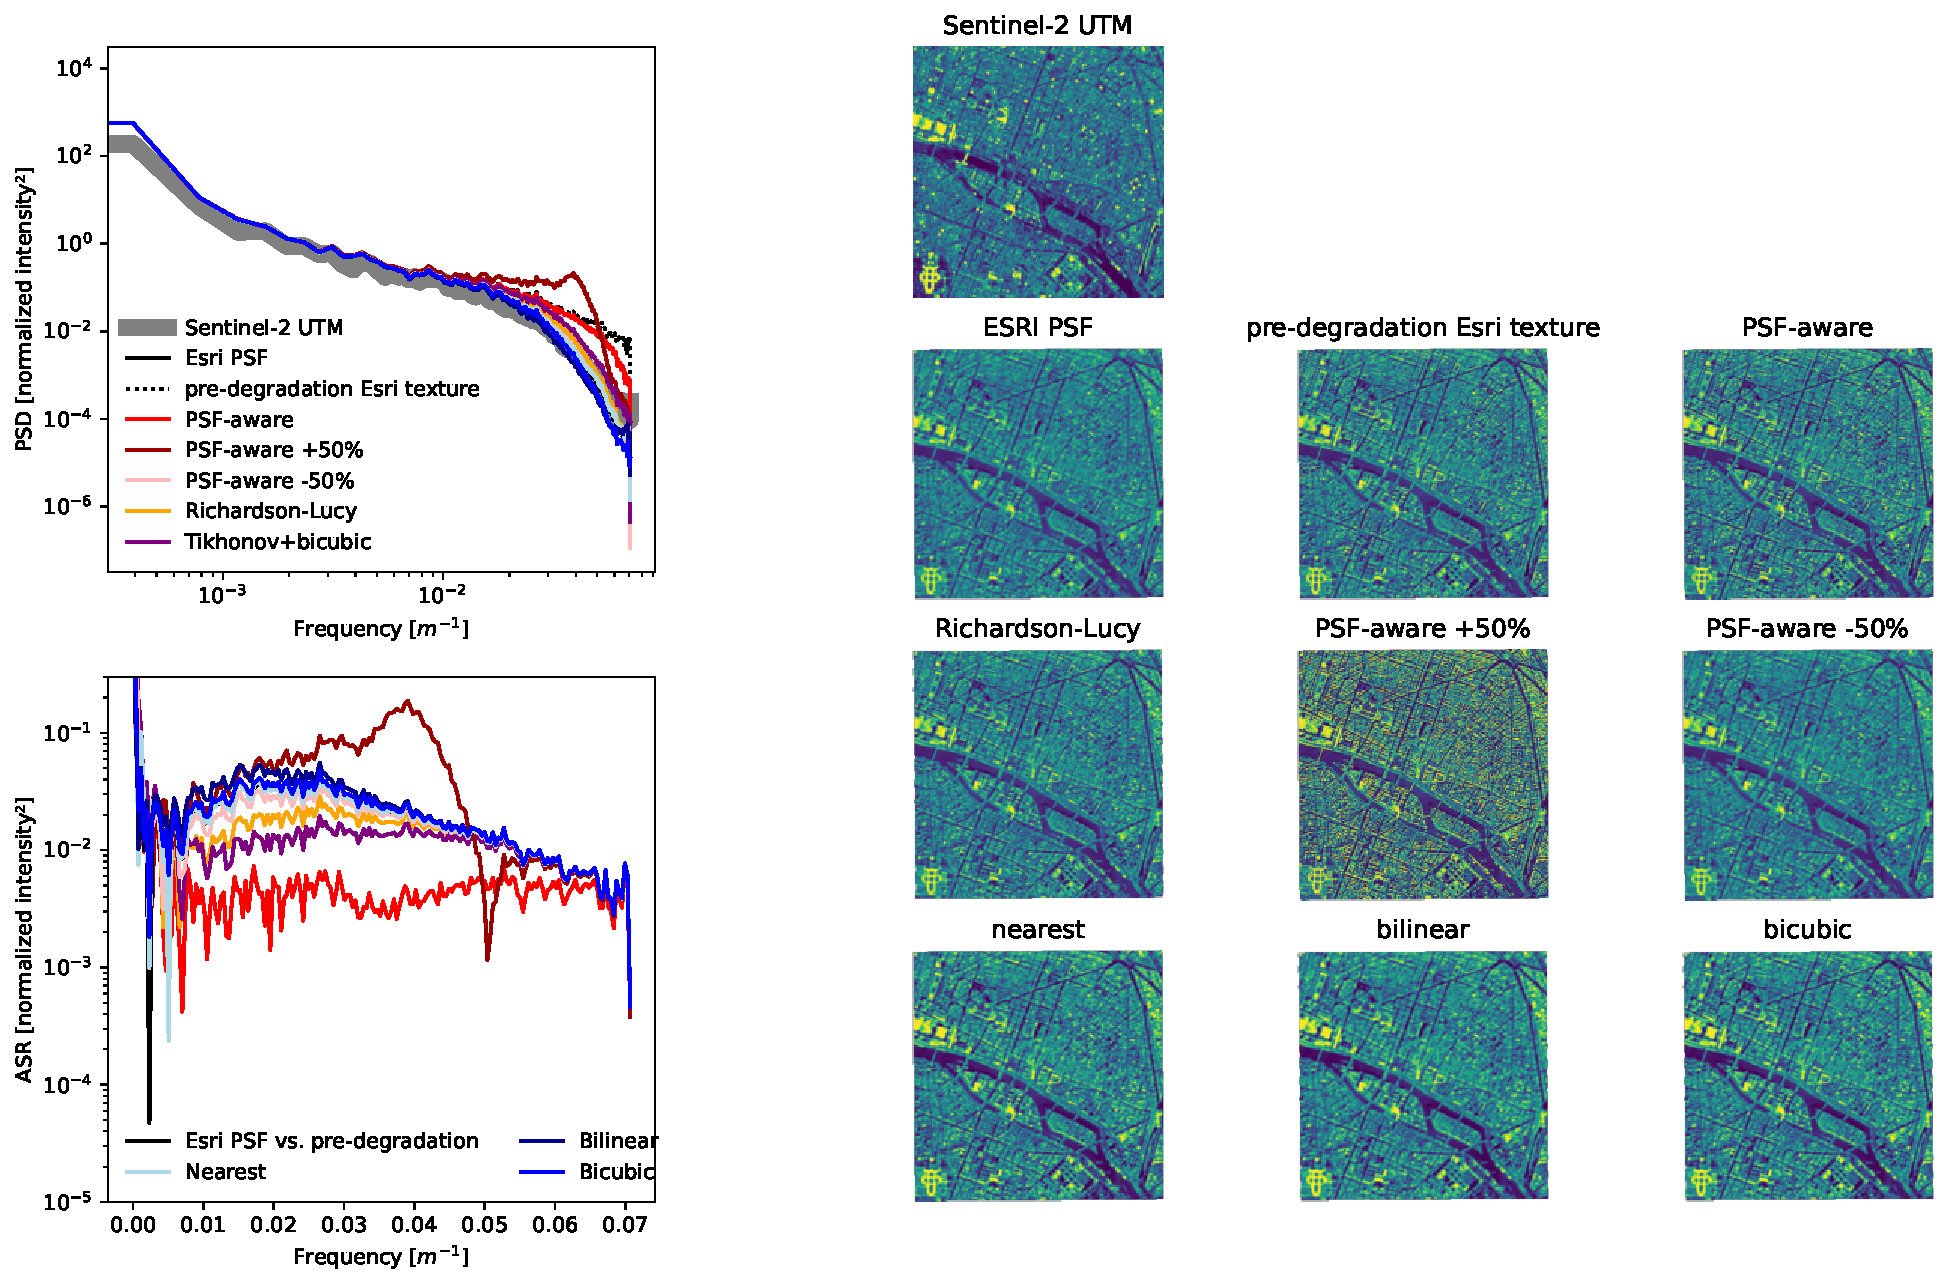
\includegraphics[width=0.98\linewidth]
    {figures/resample-test.pdf}
    \caption{Spatial and spectral diagnostics for the urban
    synthetic-detector experiment at \healpix level~20.
    \emph{Right:} reference and reconstructed fields rendered on
    the \utm grid. \emph{Top left:} isotropically averaged
    one-dimensional power spectra. \emph{Bottom left:} absolute
    spectral residuals relative to the no-\psf latent texture,
    $\left|P_{\mathrm{est}}(k)
    -P_{\mathrm{no\text{-}PSF}}(k)\right|$.
    The matched \psf-aware reconstruction is closest to the
    no-\psf reference over most of the resolved frequency range.
    Richardson--Lucy and a non-iterative Tikhonov baseline
    (Section~\ref{sec:rl_ablation}), both evaluated after the same
    bicubic-upsampled, cell-averaged \healpix regridding, give
    similar but consistently larger residuals. Overestimating
    the operator width by $50\%$ produces strong high-frequency
    amplification, whereas underestimating it primarily results
    in incomplete restoration.}
    \label{fig:synthetic_overview}
\end{figure*}

\begin{figure*}[t]
    \centering
    
\includegraphics[width=\textwidth]
    {figures/all-spectra.pdf}
    \caption{Power spectral density (PSD) and absolute spectral residuals (ASR) for the water, forest, and agriculture scenes. The matched \psf-aware reconstruction produces the smallest discrepancy across most of the resolved frequency band in all three scenes. The Richardson--Lucy solution tracks it closely but consistently remains slightly worse. The oversized \psf-aware $+50\%$ setup shows high-frequency amplification, whereas the undersized \psf-aware $-50\%$ setup stays under-corrected. These mismatch effects are less pronounced than in the urban scene, which exhibits more fine-scale, high-contrast detail.}
    \label{fig:synthetic_spectra_other}
\end{figure*}

Fig.~\ref{fig:synthetic_overview} shows the urban case. The geometric
baselines remain close to the blurred observation
and further attenuate intermediate and high frequencies. The
matched reconstruction instead shifts the spectrum toward the
latent no-\psf texture and gives the smallest absolute spectral
residual over most of the resolved band. It does not recover the
highest frequencies fully, where the observation model is weakly
constraining; the result is therefore a stable partial
deconvolution rather than complete inversion.

The mismatch spectra explain their asymmetric RMSE. The $+50\%$
operator compensates for excessive assumed attenuation and
amplifies weakly constrained high-frequency components, which a common
damping does not suppress. The $-50\%$ operator applies too little
correction and remains under-restored without the same strong
instability.

Richardson--Lucy and the non-iterative Tikhonov baseline follow the
matched spectrum closely but retain larger residuals after the same
cell-average \healpix regridding. The water, forest, and agriculture
panels of Fig.~\ref{fig:synthetic_spectra_other} reproduce the urban
ordering, with weaker mismatch effects.
Together, the four scenes link the image-domain improvement to
partial recovery of attenuated spatial variability rather than to
a uniform radiometric shift.

\subsection{Real Sentinel-2 Round-Trip Consistency}
\label{sec:roundtrip_results}

Table~\ref{tab:roundtrip_metrics} reports the
\utm--\healpix--\utm round-trip consistency between the original
Sentinel-2 observation $\mathbf{y}$ and the prediction
$\widehat{\mathbf{y}}=\mathbf{A}\widehat{\mathbf{x}}$ obtained
from the reconstructed \healpix field.

For all four scenes, the \psf-aware method yields RMSE values
between $2.8\times10^{-6}$ and $1.0\times10^{-5}$ and SSIM
between $0.99999997$ and $0.99999999$. The geometric baselines
produce substantially larger errors, with RMSE between
$8.1\times10^{-4}$ and $1.2\times10^{-2}$ and SSIM between
$0.9559$ and $0.9974$.

These results show that the inferred \healpix representation
retains the information required to reproduce the original
projected-grid observation with a residual roughly two to three
orders of magnitude smaller than the geometric baselines, under
the assumed forward model. The residual is no longer close to
floating-point precision because the matched reconstruction now
uses a light Tikhonov damping ($\lambda=0.01$,
Section~\ref{sec:exp_config}) rather than an undamped solve; the
round trip is consequently better read as a consistency and
practical reversibility test under the operating configuration
actually used elsewhere in this paper, not as independent
validation of the true instrumental \psf or recovery of an
unknown unblurred scene.

This experiment therefore complements the controlled synthetic
test: the latter evaluates partial restoration relative to a known
latent texture, whereas the Sentinel-2 round trip demonstrates
compatibility with a real operational observation.

\begin{table*}[t]
\centering
\caption{Sentinel-2 \utm--\healpix--\utm round-trip consistency.
RMSE and SSIM compare the original projected-grid observation
$\mathbf{y}$ with the prediction
$\widehat{\mathbf{y}}=\mathbf{A}\widehat{\mathbf{x}}$ reconstructed
from the \healpix field. These metrics assess observation
consistency rather than recovery of an unknown unblurred scene.
Bold indicates the best result for each scene.}
\label{tab:roundtrip_metrics}
\setlength{\tabcolsep}{5pt}
\begin{tabular}{lrrrrrrrr}
\toprule
 & \multicolumn{2}{c}{PSF-aware} & \multicolumn{2}{c}{Nearest-neighbor} & \multicolumn{2}{c}{Bilinear} & \multicolumn{2}{c}{Bicubic} \\
\cmidrule(lr){2-3}\cmidrule(lr){4-5}\cmidrule(lr){6-7}\cmidrule(lr){8-9}
Scene & RMSE & SSIM & RMSE & SSIM & RMSE & SSIM & RMSE & SSIM \\
\midrule
Urban       & $\mathbf{1.01\!\times\!10^{-5}}$ & $\mathbf{0.99999998}$ & $5.54\!\times\!10^{-3}$ & $0.9974$ & $1.21\!\times\!10^{-2}$ & $0.9559$ & $1.20\!\times\!10^{-2}$ & $0.9602$ \\
Water       & $\mathbf{3.48\!\times\!10^{-6}}$ & $\mathbf{0.99999999}$ & $1.05\!\times\!10^{-3}$ & $0.9949$ & $4.27\!\times\!10^{-3}$ & $0.9860$ & $4.12\!\times\!10^{-3}$ & $0.9883$ \\
Forest      & $\mathbf{3.28\!\times\!10^{-6}}$ & $\mathbf{0.99999999}$ & $1.08\!\times\!10^{-3}$ & $0.9912$ & $4.15\!\times\!10^{-3}$ & $0.9663$ & $4.59\!\times\!10^{-3}$ & $0.9693$ \\
Agriculture & $\mathbf{2.84\!\times\!10^{-6}}$ & $\mathbf{0.99999999}$ & $8.08\!\times\!10^{-4}$ & $0.9958$ & $3.71\!\times\!10^{-3}$ & $0.9839$ & $4.69\!\times\!10^{-3}$ & $0.9822$ \\
\bottomrule
\end{tabular}
\end{table*}

\section{Discussion}

\subsection{Observation Consistency and Partial Spatial Restoration}

The validation separates three questions: recovery relative to a
known synthetic latent field, consistency with a real projected-grid
observation, and reconstruction of real Sentinel-2 radiometry after
a controlled downscaling degradation. Across image and spectral
metrics, the geometric baselines preserve the input blur whereas
the proposed method shifts the estimate toward the latent reference.
It is therefore best interpreted as stable partial deconvolution
combined with inverse resampling, not as purely geometric regridding.

\subsection{Interpretation of the Round-Trip Experiment}
\label{sec:roundtrip_interpretation}

The round trip shows practical reversibility under the assumed
operator: a \healpix product can reproduce the four tested
projected-grid observations with residuals two to three orders of
magnitude below the geometric baselines.

This is not independent evidence of restoration. The same operator
$\mathbf A$ enters both the fit and the prediction, and roughly
$1.7\times10^{5}$ retained cells are fitted to $65\,536$
observations. A small residual is therefore expected by construction.
The random-pixel hold-out of Section~\ref{sec:holdout} checks
out-of-sample interpolation, but spatially blocked validation would
be more stringent. Likewise, Fig.~\ref{fig:psf_calibration} supports
the assumed response scale without uniquely identifying the true
instrumental \psf.

Evidence of recovery instead comes from the known latent field in
the synthetic experiments and, more cautiously, from the real-data
downscaling case study. Its primary reference is independent of the
imposed degradation, and an estimator-independent control preserves
the ranking. Degradation and reconstruction share a known matched
response in the primary arm; the anisotropic arm relaxes the
response-shape match but still uses a prescribed degradation and the
current isotropic inverse. A measured sensor MTF, calibration target,
or external higher-resolution reference would be required for fully
independent instrumental validation.

\subsection{Relation to Super-Resolution and Inversion Stability}

Using a \healpix grid finer than the native source sampling places
the method in a regime related to model-based super-resolution.
In the present experiments, the $6.22$~m \healpix cells
introduce more unknowns than the number of measurements provided
by the 10~m source pixels. These additional values are therefore
jointly inferred through the overlapping spatial-response weights;
they should not be interpreted as independent measurements at the
\healpix-cell scale.

Only spatial components sufficiently coupled to the observations
through $\mathbf A$ can be constrained. Low and intermediate
frequencies are relatively well supported, whereas the \psf
attenuates higher-frequency components and makes their inversion
increasingly sensitive to noise, geolocation errors, and
spatial-response mismatch. The method consequently aims at partial
restoration rather than complete inversion of the response.

For the matched experiment, a light Tikhonov damping of
$\lambda=10^{-3}$ is used, and stability is otherwise controlled
by the observation model and the finite conjugate-gradient
iteration. The noise sweep below separately evaluates stronger
explicit damping when weakly constrained high-frequency components
are amplified. The reconstructed
field should therefore be interpreted as a model-consistent
\healpix estimate, not as blind super-resolution or as the creation
of independent sub-pixel information. As shown below, the same
bias--variance trade-off arises under measurement noise, so no
single damping value is uniformly optimal across noise levels and
noise-correlation models.

\subsection{Robustness to Noise and Geolocation Error}
\label{sec:noise_robustness}

The primary controlled experiment of Section~\ref{sec:controlled_synthetic}
uses the deterministic forward model $\mathbf y=\mathbf A\mathbf x$ with
exact source geolocation. Appendix~\ref{app:noise_geoloc} reports three
robustness studies, kept out of the main text for length: a repeated
$\mathbf y=\mathbf A\mathbf x+\mathbf n$ sweep over five noise levels, two
noise models (white and spatially correlated), and five damping values at
the matched \psf (Appendix~\ref{sec:noise_matched}); the same sweep
repeated jointly with the $\pm50\%$ \psf-mismatch configurations of
Section~\ref{sec:psf_mismatch} (Appendix~\ref{sec:noise_psf_mismatch}); and
a sweep over independent Gaussian perturbations of each source sample's
geolocation, at $0.1$, $0.2$, and $0.4$ detector pixels
($\approx1$--$4$~m) in latitude and longitude
(Appendix~\ref{sec:geoloc_sensitivity}).

In summary: the preferred damping depends on the anticipated noise level
and correlation structure, and no single damping value is best across all
tested conditions. More surprisingly, at the arm-specific damping values
selected for the robustness comparison of
Appendix~\ref{sec:noise_psf_mismatch}, a mismatched \psf configuration can
reach a \emph{lower} noisy-image RMSE than the matched configuration once
noise dominates (all four scenes at the lowest tested SNR) -- not because
the mismatch is beneficial, but because underestimating the \psf width and
applying stronger explicit damping both act as implicit extra
regularization against noise, at the cost of the under-restoration already
characterized in Section~\ref{sec:synthetic_results}. \psf-mismatch
robustness and noise-damping robustness therefore cannot be assessed
independently. Geolocation error degrades reconstruction quality
monotonically and substantially: at $0.4$~px, RMSE increases by
$172$--$283\%$ relative to exact geolocation across the four scenes,
confirming that sub-pixel geolocation accuracy is a material requirement
for this method rather than a second-order concern.

\subsection{Model Assumptions and Generalization}
\label{sec:generalization}

The implementation uses a normalized isotropic Gaussian response.
This controlled model does not reproduce the complete Sentinel-2
image-formation chain, which can depend on band, viewing geometry,
detector, terrain, and upstream processing. The mismatch results
also show that width errors are asymmetric: underestimation mainly
under-restores, whereas overestimation can amplify poorly
constrained modes. Sensor-specific MTF or calibration information
should therefore guide the effective \psf.

The mathematical formulation accepts any non-negative local weight,
including anisotropic, band-dependent, or spatially varying
responses; in particular, the response may differ between
acquisitions or detectors. The released interface does not yet expose this
generality: it accepts only the scalar Gaussian width $s_{\psf}$.
Using a measured or tabulated kernel requires replacing the
evaluation of $g_{ij}$. The $24\times45$~m downscaling control tests
robustness when the true response shape is anisotropic but the inverse
model remains isotropic; it does not validate native anisotropic-kernel
support.

The detailed noise and round-trip diagnostics use one illustrative patch
per scene class. Their cell-level metrics are case studies, not independent
population estimates. The two controls on the downscaling experiment are
likewise four-patch studies: the geometric control removes the shared
estimator from the reference and preserves the ranking, and the anisotropic
control probes one additional imposed response shape.

The downscaling result itself is no longer of that kind. Section
\ref{sec:real_downscale_multiregion_results} repeats it over 38 independent
real Sentinel-2 regions on the same site list as the synthetic multi-region
validation, with the region as the statistical unit. What that establishes is
diversity of scene and geography, not of instrument: a single sensor, band and
resolution ratio are involved throughout, and the reconstruction always
assumes the response actually used to degrade the observation.

Restricting the evaluation to B04 is a deliberate scope limit rather than a
convenience, and it is worth saying what it does and does not cost. The four
$10$~m MSI bands (B02, B03, B04, B08) share one focal plane and one optical
train, and their MTF-at-Nyquist specifications lie within a few percent of
each other~\cite{esa_s2_mtf_technical_guide}; the effective response width
calibrated in Section~\ref{sec:psf_calibration} would therefore shift by far
less than the $\pm20\%$ that Section~\ref{sec:real_downscale_multiregion_results}
shows the ranking tolerates. What genuinely differs between these bands is
scene content, not instrument response -- and scene content is the axis this
paper already varies deliberately, across four classes and 38 regions. A
second $10$~m band would thus add samples along an axis already sampled while
leaving the untested axes untouched. The scope limit that matters is the one
we cannot buy this way: the $20$~m and $60$~m bands, which are resampled
differently on board and would change the resolution ratio, and other sensors
entirely.

Which regions survive is set by Sentinel-2 availability -- catalogue coverage,
cloud, granule edges -- through criteria evaluated before any reconstruction.
That cannot bias the comparison between methods, since all methods see the
same surviving patches, but it does mean the 38 regions are not a random
sample of the four scene classes, and the two excluded sites were removed for insufficient overlap between
reference and reconstruction, not for anything about the scene.

Broader validation should vary sensor, band, target resolution,
response shape, noise, geolocation, and patch boundaries, and cover
conditions excluded here, including clouds, snow and ice, open
ocean, mountains, coasts, and incomplete observations.

\subsection{Outlook: Multi-Observation Fusion and Irregular Sampling}
\label{sec:outlook_fusion}

Because each operator row requires only a sample location, value,
and spatial response, observations need not form a regular raster or
come from one acquisition. Overlapping images could be combined in
one inverse problem against a shared \healpix field, turning
redundant Sentinel-2 UTM/MGRS coverage into additional constraints
rather than separate mosaicked estimates~\cite{bauer2023wasting}.

More generally, acquisition or detector $m$ could be represented as
\begin{equation}
\mathbf y_m = \mathbf A_m(\boldsymbol\theta_m)\mathbf x
             + \mathbf T_m\boldsymbol\alpha_m + \mathbf n_m,
\label{eq:multi_observation_outlook}
\end{equation}
where $\mathbf A_m$ contains its geolocation and possibly asymmetric
or spatially varying \psf parameters $\boldsymbol\theta_m$, while
$\mathbf T_m\boldsymbol\alpha_m$ represents gains, offsets, or other
instrumental templates. Stacking these blocks would allow all
observations to constrain the same field $\mathbf x$, with their
noise covariances supplying statistically appropriate relative
weights. Data redundancy could then support joint estimation of
selected instrumental parameters, following the general map-making
logic exemplified by SRoll2~\cite{delouis2019sroll2}. Such a joint fit
is not implemented or evaluated here and would require explicit
identifiability tests, priors, and uncertainty propagation.

The same construction could ingest native irregular or wide-swath
samples such as Sentinel-3 OLCI/SLSTR or SWOT HR without an
intermediate raster. Neither multi-acquisition fusion nor irregular
sampling is evaluated here; both require dedicated baselines and
uncertainty analysis. Direct stacking is appropriate for measurements
of the same latent physical quantity; cross-band or time-separated
fusion additionally requires a spectral or temporal observation
model rather than an assumption that the latent field is unchanged.

\subsection{Implications for HEALPix Earth-Observation Data Cubes}
\label{sec:hpx_datacube_implications}

The formulation links sensor observations to a global, equal-area,
hierarchical support through an explicit forward model. The common
storage grid should therefore not be confused with the effective
resolution of each observation. A support finer than the native
grid introduces spatial redundancy in exchange for a non-overlapping
global index, equal-area cells, and hierarchical access; storage and
compression are not evaluated here.

In this interpretation, \healpix supplies the common latent support,
but does not require the inputs to be pre-convolved to one common
\psf. Each acquisition can retain its own response operator while
contributing to a single PSF-aware estimate. This preserves more of
the available information than unconditional smoothing to the
poorest resolution and makes the effective resolution a property of
the combined observation operator, not merely of the output cell
size. Future work should therefore accompany fused products with
cell- or region-dependent uncertainty and effective-resolution
diagnostics derived from the normal operator or its approximations.

On the tested NVIDIA A100 80GB PCIe system, the median core runtime
(operator construction plus matrix-free conjugate-gradient solve)
over 357 timed $256\times256$ patches was $0.315\,\mathrm{s}$ for
the matched configuration (interquartile range
$0.312$--$0.320\,\mathrm{s}$). The $-50\%$ and $+50\%$ mismatch
configurations required $0.198\,\mathrm{s}$ and $0.519\,\mathrm{s}$,
respectively, because their retained neighbourhoods differ. For
comparison, nearest-neighbor, bilinear, and bicubic interpolation
required $0.123\,\mathrm{s}$, $0.109\,\mathrm{s}$, and
$0.764\,\mathrm{s}$ in this implementation.

Operator construction accounts for $0.274\,\mathrm{s}$ ($87\%$) of
the matched core runtime and the solve for $0.040\,\mathrm{s}$
($13\%$). Operators depend on geometry rather than image values and
can therefore be reused for acquisitions sharing a footprint. The
separate detector-grid projection used only for spectral diagnostics
costs about $1.76\,\mathrm{s}$ and is excluded from these resampling
times. Regional deployment will still require parallel construction,
chunk scheduling, and preconditioning.

For the matched configuration ($q=22$), the sparse operator has a
median of $1{,}441{,}792$ non-zero coefficients and retains
$171{,}259$ \healpix cells. Peak GPU memory had a median of
$1021\,\mathrm{MiB}$ and a maximum of $1382\,\mathrm{MiB}$. Peak host
resident-set size was $18{,}197\,\mathrm{MiB}$ (maximum
$18{,}276\,\mathrm{MiB}$), but that figure measures the whole validation
process -- cached scene arrays, spectral records and the accumulated metric
tables -- rather than the resampler, so it is an upper bound for a batch job
and not the memory required for one reconstruction. Across the run the
post-cleanup resident set drifted by $-0.16\,\mathrm{MiB}$ per patch, i.e.\
no accumulation.

A single batch-scaling sweep on the same system
(Appendix~\ref{app:throughput_scaling}) observed an
$8.6\times$--$10.0\times$ lower amortized cost when one operator was
shared across repeated acquisitions. At batch size 2048, the observed
throughput was $83{,}347$~patches/h; distinct footprints do not permit
this reuse. Because batch sizes were not replicated, these values are
descriptive observations rather than estimates with run-to-run
uncertainty.

\section{Conclusion}

We introduced \texttt{healpix-resample}, a \psf-aware framework that
maps projected Earth-observation imagery onto \healpix through a
sparse, matrix-free weighted inverse problem. Unlike geometric
interpolation, it retains an explicit relationship between the
reconstructed field, sampling geometry, and assumed spatial response.

In the four controlled scenes, the matched reconstruction reduced
blur-induced RMSE by $17$--$22\%$ and partially recovered attenuated
frequencies. Across 40 regions and 358 valid patches, the
region-cluster bootstrap interval was positive in every scene class
($15.4$--$19.6\%$), and the method outperformed all five
multi-region comparators on every patch. The adopted $12.5$~m B04
response is consistent with the observed spectral slopes and the
published MSI MTF range, but is not identified as a unique processed
Level-2A \psf. Width mismatch experiments further show that
over-restoration amplifies weakly constrained frequencies.

On one independently selected patch from each of the same 40 regions,
the matched reconstruction also outperformed fixed-configuration
Tikhonov and Richardson--Lucy two-stage pipelines in all 40 cases;
the paired region-bootstrap intervals excluded zero in every scene
class. This strengthens the comparison with conventional
deconvolution while not constituting a ranking against per-region
optimized baselines.

On real Sentinel-2 data, near-zero round-trip residuals demonstrate
internal consistency under the assumed model, not recovery of a
latent high-resolution truth. The downscaling experiment supplies that
missing evidence: against a reference built independently of the imposed
degradation, the \psf-aware reconstruction has the lowest RMSE in
\emph{all 38} real Sentinel-2 regions tested, against each of four
competitors (exact two-sided sign test $p=7.3\times10^{-12}$), with mean
paired margins from $10.3\%$ over water to $17.9\%$ over forest relative
to Richardson--Lucy, the strongest comparator throughout. Those regions are
the same sites as the synthetic multi-region validation, so the two
experiments are comparable in coverage. On the four-scene version of the
test the ranking also survives an estimator-independent geometric reference
and an anisotropic $24\times45$~m degradation inverted with an isotropic
model. The scope is scene and geographic diversity, not instrument
diversity: one sensor, one band, one resolution ratio, and a reconstruction
that always assumes the response used to degrade the observation. Noise
experiments show that no
single damping value is optimal: stronger $\lambda$ becomes useful as
white-noise amplitude increases, but adds bias for clean or correlated
cases. Selecting $\lambda$ dynamically from noise covariance,
resolution ratio, and scene structure is therefore left to future
work. Geolocation errors remain a separate material limitation.

The matched core runtime was $0.315\,\mathrm{s}$ per
$256\times256$ patch on an NVIDIA A100, dominated by reusable
operator construction. Exact area-integral conservation is available
through optional methods evaluated separately. Scaling to regional or
global production will require operator reuse, parallel construction,
chunk scheduling, storage design, and validation on additional
sensors and acquisition conditions.

Beyond the single-sensor experiments reported here, the structural
consequence of the forward-model formulation is that observations
with different sampling patterns and spatial responses can be posed
as blocks of one map-making problem on a shared \healpix support.
This opens a path toward PSF-aware multi-detector fusion, uncertainty
and effective-resolution products, and---where redundancy and
identifiability permit---joint fitting of selected instrumental
errors. These capabilities remain prospective and are not claimed as
validated results of the present study.

\appendices

\section{Measurement Noise and Geolocation Robustness}
\label{app:noise_geoloc}

\subsection{Noise Sensitivity Under the Matched \psf}
\label{sec:noise_matched}

We complement the deterministic experiment of
Section~\ref{sec:controlled_synthetic} with a repeated
$\mathbf y=\mathbf A\mathbf x+\mathbf n$ experiment in which
$\mathbf n$ is either white Gaussian noise or spatially correlated
Gaussian noise obtained by Gaussian smoothing with a width of
$1.5$ source pixels and subsequent variance renormalization. Five
nominal SNR levels, from 100 to 5, are used to generate the
perturbations, but the analysis is reported against the resulting
absolute input-noise standard deviation $\sigma_n$. This avoids
treating a fixed SNR as the same noise amplitude in scenes having
different radiometric variance.

We test $\lambda\in\{0,10^{-3},10^{-2},10^{-1},1\}$ on the four
scenes, using ten independent noise realizations per configuration.
The same realization is shared across the five damping values so
that their comparison is paired. To retain the bias introduced by
regularization, every noisy result is compared with the same clean,
undamped reference. We define the excess reconstruction error as

\begin{equation}
E_{\lambda}(\sigma_n)=
\sqrt{\max\!\left\{
\operatorname{RMSE}_{\mathrm{noise},\lambda}^{2}
-\operatorname{RMSE}_{\mathrm{clean},0}^{2},\,0
\right\}}.
\label{eq:noise_excess_error}
\end{equation}

Using the clean result at the corresponding $\lambda$ instead would
remove the regularization bias and make progressively stronger
damping appear artificially favourable. Equation~\eqref{eq:noise_excess_error}
instead exposes the complete trade-off relative to the noise-free,
undamped reconstruction.

\begin{figure}[t]
\centering

\includegraphics[width=\columnwidth]{noise_transfer_loglog.pdf}
\caption{Noise sensitivity across the four synthetic scenes, matched
\psf. The abscissa is the absolute standard deviation $\sigma_n$ of
the injected measurement noise, rather than the scene-dependent SNR.
The ordinate is the excess reconstruction error of
Eq.~\eqref{eq:noise_excess_error}, relative to the common clean
$\lambda=0$ result. Colours identify the damping value and marker
shapes identify the scene. Points show the mean over ten paired
noise realizations and error bars show one standard deviation
(often smaller than the marker). White and spatially correlated
noise are shown separately. Every solve, including $\lambda=0$, uses
a zero CG initial vector and at most 14 iterations.}
\label{fig:noise_transfer}
\end{figure}

Figure~\ref{fig:noise_transfer} shows that the appropriate damping
depends on the anticipated noise level. For white noise, the lowest
tested amplitudes favour little or no explicit damping, whereas the
preferred value shifts toward $\lambda=10^{-1}$ or $1$ as
$\sigma_n$ increases. Strong damping is therefore useful when
white-noise amplification dominates, but its non-zero error floor
becomes detrimental for cleaner data. The transition varies across
scenes, consistent with differences in their spatial spectra and in
the fraction of fine-scale structure that is only weakly constrained
on a $6.22$~m target grid from 10~m measurements.

For the correlated-noise model tested here, $\lambda=0$ gives the
lowest excess error across all four scenes and all five noise
levels. Increasing $\lambda$ then adds more bias than the amount of
correlated error it removes. This result is specific to the chosen
correlation scale and to the common zero-initialized, at-most-14-step
CG rule. In particular, it does not establish a unique undamped
solution and should not be generalized to arbitrary stopping rules
or noise covariances.

The ordinate in Fig.~\ref{fig:noise_transfer} should not be read as
an estimate of sensor noise alone. It combines propagation of the
injected perturbation with the response of weakly constrained
small-scale degrees of freedom and, for $\lambda>0$, the retained
regularization bias. This is precisely why an absolute noise scale
is more interpretable here than SNR alone. In principle, $\lambda$
could be selected from an expected noise amplitude and covariance,
the source-to-target resolution ratio, and local scene structure.
The present paper does not attempt such dynamic selection: the main
matched comparison retains the fixed $\lambda=10^{-3}$ configuration.
Developing and validating a noise-adaptive rule, for example through
a discrepancy principle, generalized cross-validation, or a
hierarchical noise model, is left to a dedicated study. This
experiment remains limited to one patch per scene type
(Section~\ref{sec:generalization}).

A multi-date extension of the real-data downscaling protocol would
provide realistic sensor and atmospheric perturbations. It is left
for future work because it requires cloud-free repeat coverage and a
separate treatment of genuine surface change. Repeating only the
round trip would test self-consistency rather than reconstruction
quality.

\subsection{Interaction Between Noise and \psf Mismatch}
\label{sec:noise_psf_mismatch}

The sweep of Appendix~\ref{sec:noise_matched} uses only the matched
\psf configuration. We repeat it, at the same five SNR levels and
ten paired realizations, for the $\pm50\%$ mismatch configurations
of Section~\ref{sec:psf_mismatch}, each evaluated at its own
per-arm damping ($\lambda=0.01$ for matched and $-50\%$, $\lambda=0.1$
for $+50\%$). These values define a separate arm-specific robustness
comparison selected from the damping sweep; they are not the common
$\lambda=10^{-3}$ configuration of Table~\ref{tab:synthetic_metrics}.
This directly tests the \psf-mismatch configurations jointly with
measurement noise rather than only at the matched configuration.

\begin{figure}[t]
\centering

\includegraphics[width=\columnwidth]{noise_psf_mismatch_summary.pdf}
\caption{RMSE against the pre-degradation reference, under white and
spatially correlated noise, for the matched and $\pm50\%$
mismatched \psf configurations, each at its own per-arm damping.
Points are the mean over the four scenes at each SNR level.}
\label{fig:noise_psf_mismatch}
\end{figure}

Fig.~\ref{fig:noise_psf_mismatch} summarizes the resulting
behaviour across SNR levels, and
Table~\ref{tab:noise_psf_mismatch} reports the RMSE against the
pre-degradation reference under white noise for the two extreme tested
SNR levels. At the mild-noise end (SNR$=100$, close to the
noise-free case), the matched configuration remains the best in
every scene, consistent with Section~\ref{sec:synthetic_results}.
At the severe-noise end (SNR$=5$), this ranking reverses in all
four scenes: a mismatched configuration achieves a \emph{lower}
RMSE than the matched configuration. This is not evidence that
\psf mismatch is beneficial. Two confounded effects are at play:
underestimating the \psf width leaves the inversion
under-correcting the blur, which incidentally behaves like extra
implicit regularization against noise; and the $+50\%$ arm is
evaluated at a ten-times stronger explicit damping ($\lambda=0.1$
instead of $0.01$) specifically because that configuration is
otherwise the most ill-conditioned; this arm-specific choice is used
only for the robustness comparison and likewise suppresses noise at
the cost of bias. Both effects trade restoration accuracy for noise
robustness. Under the common $\lambda=10^{-3}$ comparison, both width
mismatches already degrade the noise-free reconstruction relative to
the matched configuration (Table~\ref{tab:synthetic_metrics}); the
present arm-specific damping adds a second, explicit bias--variance
trade-off. The practical implication is
that \psf-mismatch robustness and noise-damping robustness cannot
be tuned independently: a damping value chosen only from an assumed
noise level, or a \psf width chosen only from a clean-data accuracy
target, can silently interact in either direction.

\begin{table}[t]
\centering
\caption{RMSE against the pre-degradation reference, white noise, at the
two extreme tested SNR levels, for the matched and $\pm50\%$ \psf
configurations at their respective per-arm damping. Bold indicates
the lowest RMSE in each row.}
\label{tab:noise_psf_mismatch}
\begin{tabular}{llrrr}
\toprule
Scene & SNR & Matched & $-50\%$ & $+50\%$ \\
\midrule
Agriculture & 5   & 0.0694 & \textbf{0.0354} & 0.0360 \\
Agriculture & 100 & \textbf{0.0160} & 0.0225 & 0.0186 \\
Forest      & 5   & 0.0628 & 0.0407 & \textbf{0.0395} \\
Forest      & 100 & \textbf{0.0246} & 0.0333 & 0.0295 \\
Urban       & 5   & 0.0962 & 0.1014 & \textbf{0.0907} \\
Urban       & 100 & \textbf{0.0693} & 0.0977 & 0.0855 \\
Water       & 5   & 0.0646 & 0.0399 & \textbf{0.0385} \\
Water       & 100 & \textbf{0.0218} & 0.0314 & 0.0267 \\
\bottomrule
\end{tabular}
\end{table}

\subsection{Geolocation Sensitivity}
\label{sec:geoloc_sensitivity}

We also test sensitivity to source-sample geolocation error.
Independent Gaussian perturbations are applied to each source
sample's longitude and latitude before the observation operator is
built, at three levels expressed in native detector pixels
($0.1$, $0.2$, $0.4$~px, i.e.\ approximately $1$, $2$, and $4$~m at
the $10$~m Sentinel-2 B04 sampling used throughout), with ten
independent realizations per level and per scene, at the matched
\psf and $\lambda=0.01$. Because the operator's geometry itself
depends on the (perturbed) source positions, the operator is
rebuilt for every realization rather than reused. For each scene,
the ten realizations perturb the same base patch; they are not ten
independently sampled geographic scenes.

\begin{figure}[t]
\centering

\includegraphics[width=\columnwidth]{geolocation_sensitivity.pdf}
\caption{RMSE against the pre-degradation reference as a function of
geolocation jitter standard deviation, for the matched \psf
configuration ($\lambda=0.01$). Error bars show one standard
deviation over ten perturbations of one base patch per scene.}
\label{fig:geoloc_sensitivity}
\end{figure}

Fig.~\ref{fig:geoloc_sensitivity} shows the resulting RMSE as a
function of jitter amplitude, and
Table~\ref{tab:geoloc_sensitivity} reports the relative RMSE
increase over the exact-geolocation baseline. Degradation is
monotonic and substantial: at $0.1$~px ($\approx1$~m) RMSE already
increases by $14$--$27\%$, and at $0.4$~px ($\approx4$~m) it
increases by $172$--$283\%$, more than doubling or tripling the
reconstruction error in every scene. Unlike the noise sweep above,
no damping-based mitigation is tested here: the mismatch is purely
geometric, between the assumed and the true source-sample location,
and is not the kind of error that regularization against noise
suppresses. This confirms that sub-pixel geolocation accuracy is a
material requirement for the method, not a second-order concern,
and motivates the geolocation-correction terms outlined as future
work in Section~\ref{sec:generalization}.

\begin{table}[t]
\centering
\caption{RMSE increase relative to exact geolocation ($\sigma=0$),
matched \psf, $\lambda=0.01$, mean over ten realizations per level.}
\label{tab:geoloc_sensitivity}
\begin{tabular}{lrrr}
\toprule
Scene & $0.1$~px & $0.2$~px & $0.4$~px \\
\midrule
Agriculture & $+27\%$ & $+101\%$ & $+283\%$ \\
Forest      & $+15\%$ & $+61\%$  & $+184\%$ \\
Urban       & $+14\%$ & $+56\%$  & $+172\%$ \\
Water       & $+17\%$ & $+69\%$  & $+202\%$ \\
\bottomrule
\end{tabular}
\end{table}

\section{Throughput and Batch-Scaling Benchmark}
\label{app:throughput_scaling}

Section~\ref{sec:hpx_datacube_implications} times one patch at a time.
A dedicated notebook benchmark on the same NVIDIA A100 80GB PCIe
system as
Section~\ref{sec:hpx_datacube_implications} reuses patches cached
by the multi-region validation and times batch sizes from 1 to 2048
under three
regimes: one operator shared across a batch of repeated acquisitions
of the same footprint (independent per-item radiometric noise only);
the same footprint with the operator rebuilt every item, a naive
baseline isolating the benefit of reuse; and a batch of real,
distinct cached patches (operator necessarily rebuilt each time).
Each regime and batch size was run once, so the results characterize
the observed scaling sweep rather than repeat-to-repeat uncertainty;
no confidence interval across independent benchmark runs can be
reported.

\begin{figure}[t]
\centering

\includegraphics[width=\columnwidth]{throughput_scaling_curve.pdf}
\caption{Observed wall time per patch in one batch-scaling sweep, for
the three regimes described in the text.}
\label{fig:throughput_scaling}
\end{figure}

Figure~\ref{fig:throughput_scaling} shows the observed scaling curve.
Over the 8190 timed builds, per-item operator construction
has a median of $0.326$~s with a tight central spread
(interquartile range $0.323$--$0.330$~s), but that figure is
dominated by the large batches: the per-batch-size medians fall
from $0.69$--$1.20$~s at batch sizes 1--256 to a stable
$0.325$~s at 512 and above, and 500 of the 8190 builds exceed 1~s
(the slowest reaching $3.7$~s). The early, smaller batches are
therefore measurably slower, consistent with warm-up and with
contention on a shared accelerator, and the per-batch figures
should be read accordingly. The solve is highly reproducible at a
median of $0.041$~s regardless of batch size. Sharing one operator
across a batch amortizes construction away: at batch size 2048,
the shared-operator regime reaches $0.043$~s/patch
($83{,}347$~patches/h), against $0.372$~s/patch ($9{,}679$/h) for
the same footprint rebuilt every time and $0.430$~s/patch
($8{,}370$/h) for 2048 draws over the 360-patch cache pool (with
replacement beyond 360; all 360 patches were drawn at least once).
This single sweep gives an observed $8.6\times$--$10.0\times$ speedup from
operator reuse, quantifying the argument of
Section~\ref{sec:hpx_datacube_implications}: repeated acquisitions of
the same footprint benefit substantially from reuse, while batches of
distinct geographic patches do not.

\section{Exact Conservation of Area-Integrated Quantities}
\label{app:conservative}

The main text addresses spatial fidelity under an assumed sensor
response. Some applications impose a different requirement:
preserving an area-integrated quantity exactly when a field is
transferred between grids. This is essential for fluxes used in
budget calculations, boundary conditions, and coupling terms in
Earth-system models.

This appendix presents two optional conservation paths implemented
in \texttt{healpix-resample}. The first adds a global linear
constraint to the smooth \psf-aware reconstruction. The second is
a purely algebraic hard-binning operator that conserves the
discrete area-weighted source sum by construction. Neither method
is used in the Sentinel-2 experiments of the main text. Their
purpose is to support applications for which integrated
conservation, rather than spatial restoration alone, is required.


\subsection{Relation to Conservative Remapping Tools}
\label{sec:related_conservative}

Conservative remapping is well established in climate and
Earth-system modeling. SCRIP, ESMF, xESMF, and TempestRemap
construct conservative weights from intersections between
finite-area source and target cells
\cite{jones1999scrip,hill2004esmf,zhuang2020xesmf,
ullrich2015tempestremap}.

The hard-binning method introduced below addresses the same
conservation objective but uses a different construction: source
samples are treated as area-weighted points and assigned to a
single \healpix cell. It therefore conserves the resulting
discrete weighted sum exactly, but it is not a polygon-overlap
remapper. The constrained \psf-aware method instead preserves the
smooth kernel-based reconstruction while imposing a prescribed
global integral.


\subsection{Optional Flux-Conservation Constraint}
\label{sec:conservative_constraint}

The correction defined by Eq.~\eqref{eq:correction_system}
minimizes an observation-space residual but does not guarantee
preservation of an area-integrated source quantity. Let $a_i$ be
the area, or more generally the extensive weight, associated with
source sample $i$.

For a complete global remapping, or whenever the total area of the
retained target support equals that of the source support,
conservation can be expressed as equality of the source and target
area-weighted means. Because the retained \healpix cells are
equal-area, this becomes

\begin{equation}
\frac{1}{M}\sum_{j=1}^{M}\widehat x_j
=
\frac{\sum_{i=1}^{N}y_i a_i}
     {\sum_{i=1}^{N}a_i}.
\label{eq:flux_constraint}
\end{equation}

The same source weights $a_i$ are used in the construction of
$\mathbf B$ and in Eq.~\eqref{eq:flux_constraint}, ensuring a
consistent area convention.

Let $\mathbf c=\mathbf 1_M$ and define

\begin{equation}
g
=
F-\mathbf c^{\mathsf T}\mathbf x_{\mathrm{ref}},
\end{equation}

where $F$ is the right-hand side of
Eq.~\eqref{eq:flux_constraint} multiplied by $M$. The constrained
correction minimizes the weighted objective of
Eq.~\eqref{eq:weighted_variational} subject to

\begin{equation}
\mathbf c^{\mathsf T}\boldsymbol\delta_{\mathrm{cons}}=g.
\end{equation}

Introducing a Lagrange multiplier $\nu$ gives

\begin{equation}
\mathbf H\boldsymbol\delta_{\mathrm{cons}}
=
\mathbf B\mathbf r_{\mathrm{ref}}
+
\nu\,\mathbf D_x^{-1}\mathbf c,
\label{eq:constrained_system}
\end{equation}

with

\begin{equation}
\mathbf H=\mathbf B\mathbf A+\lambda\mathbf I.
\end{equation}

By linearity,

\begin{equation}
\boldsymbol\delta_{\mathrm{cons}}
=
\boldsymbol\delta+\nu\mathbf w,
\qquad
\mathbf H\mathbf w=\mathbf D_x^{-1}\mathbf c,
\end{equation}

where $\boldsymbol\delta$ is the unconstrained correction. The
multiplier is then

\begin{equation}
\nu
=
\frac{
g-\mathbf c^{\mathsf T}\boldsymbol\delta
}{
\mathbf c^{\mathsf T}\mathbf w
}.
\label{eq:conservative_multiplier}
\end{equation}

The right-hand side of the auxiliary system is
$\mathbf D_x^{-1}\mathbf c$, rather than $\mathbf c$, because the
minimum-distortion correction is defined in the
$\mathbf D_x$-weighted metric. Computing $\mathbf w$ requires one
additional matrix-free conjugate-gradient solve with the same
operator and weighted inner product as the unconstrained
correction. The asymptotic cost remains
$\mathcal O(n_{\mathrm{it}}qN)$, with approximately twice the
iteration budget.

Once $\boldsymbol\delta$ and $\mathbf w$ have been computed,
Eq.~\eqref{eq:conservative_multiplier} imposes the scalar
constraint algebraically. The remaining conservation error is
therefore governed primarily by floating-point evaluation of the
global sums and correction. The conjugate-gradient accuracy
instead controls how closely $\mathbf w$ approximates the
minimum-distortion correction direction.

\subsection{Hard-Binning Conservative Resampling}
\label{sec:hard_binning}

When a smooth reconstructed field is not required, exact
conservation can be obtained without a spatial kernel or an
iterative solve. The
\texttt{ConservativeResampler} assigns each source sample to one
\healpix cell and conserves the resulting discrete weighted sum.

Let $\mathcal S_k$ be the set of source samples whose locations
fall inside target cell $k$. The sets $\{\mathcal S_k\}$ form a
disjoint partition of the retained source samples. The extensive
quantity assigned to cell $k$ is

\begin{equation}
h_k
=
\sum_{i\in\mathcal S_k}v_i a_i,
\label{eq:hardbin_forward}
\end{equation}

and a coverage-weighted mean can be mapped back to the contributing
source samples as

\begin{equation}
\widehat v_i
=
\frac{h_k}{A_k},
\qquad
A_k
=
\sum_{i\in\mathcal S_k}a_i,
\qquad
i\in\mathcal S_k.
\label{eq:hardbin_inverse}
\end{equation}

Conservation follows directly from the partition:

\begin{equation}
\sum_k h_k
=
\sum_k\sum_{i\in\mathcal S_k}v_i a_i
=
\sum_{i=1}^{N}v_i a_i.
\label{eq:hardbin_identity}
\end{equation}

This identity holds up to floating-point summation error and is
independent of the source-grid regularity or target \healpix
resolution.

The quantity $h_k$ is an extensive cell total. The normalization
$A_k$ in Eq.~\eqref{eq:hardbin_inverse} is the total source weight
assigned to cell $k$, not necessarily the geometric area of the
complete \healpix cell. Consequently,
Eq.~\eqref{eq:hardbin_inverse} defines a source-coverage-weighted
density and ensures a self-consistent back projection; it should
not be interpreted as a polygon-overlap estimate of the complete
target-cell mean.

Hard binning is exact and inexpensive but does not model a spatial
response and produces a piecewise-constant representation. The
constrained \psf-aware method instead retains a smooth,
kernel-based reconstruction at the cost of an additional iterative
solve. The appropriate choice therefore depends on whether the
downstream application prioritizes a spatial-response model,
discrete conservation, or both.

\subsection{ERA5 Experimental Setup}
\label{sec:era5_experiment}

The conservation methods were evaluated using ERA5 surface
sensible heat flux (\texttt{sshf}), for which the global
area-integrated total is physically meaningful. Data were obtained
from the ECMWF \texttt{reanalysis-era5-complete} archive
(\texttt{stream=enda}) for the ten ensemble members
\texttt{number=0--9}, at forecast steps 3 and 6~h, on the native
N256 reduced Gaussian grid containing 348{,}528 points.

Because \texttt{sshf} is accumulated, the mean flux over the
3--6~h interval was obtained as

\begin{equation}
\mathrm{flux}
=
\frac{
\mathrm{sshf}(6\,\mathrm h)-\mathrm{sshf}(3\,\mathrm h)
}{
3\times3600\,\mathrm s
}.
\label{eq:deaccum}
\end{equation}

The resulting values span approximately
$[-350,310]\,\mathrm{W\,m^{-2}}$ across the ensemble.

Per-sample area weights $a_i$ were constructed from midpoint
latitude boundaries and the longitude spacing of each reduced
Gaussian-grid ring. By construction, their sum reproduces the
sphere area $4\pi R^2$ to floating-point precision. These weights
are required because the source points are not exactly equal-area:
the largest associated area is approximately $3.6$ times the
smallest.

Both methods target a nested level-6 \healpix grid
($N_{\mathrm{side}}=64$, $K=49{,}152$ cells). Hard binning uses
only the source values, coordinates, and area weights. The
constrained kernel-based reconstruction uses nine target
neighbours per source sample, a Gaussian scale tied to the
level-6 pixel size, $\lambda=10^{-3}$, at most 200
conjugate-gradient iterations, and a relative residual tolerance
of $10^{-8}$. The conservation constraint is enabled through
\texttt{conservative=True} and requires the additional solve
described above.

For ensemble member $b$, the conservation metric is

\begin{equation}
\varepsilon_b
=
\frac{
\left|\widehat F_b-F_b\right|
}{
\left|F_b\right|
},
\qquad
F_b
=
\sum_{i=1}^{N}\mathrm{flux}_{b,i}a_i,
\label{eq:conservation_error}
\end{equation}

where $\widehat F_b$ is the total recovered from the remapped
representation. For hard binning,
$\widehat F_b=\sum_k h_{b,k}$. For the constrained reconstruction,
it is obtained from the target mean and the total source area,
consistently with Eq.~\eqref{eq:flux_constraint}.


\subsection{Results: Flux Conservation on ERA5 Data}
\label{sec:era5_results}

\begin{figure}[t!]
\centering
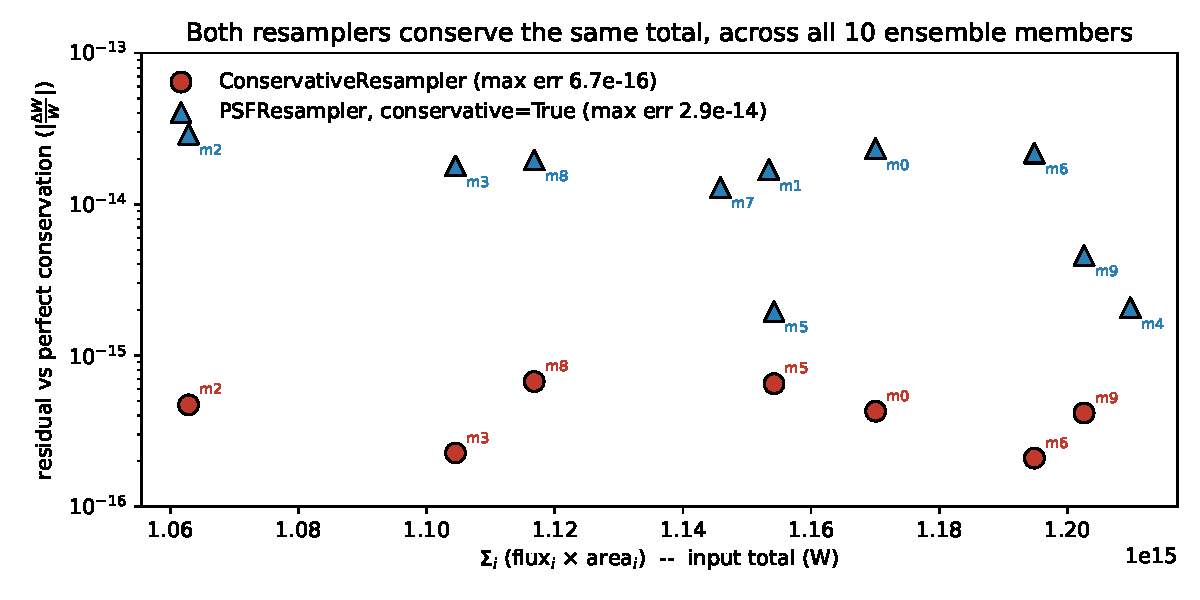
\includegraphics[width=\columnwidth]{conservative_proof.pdf}
\caption{Relative error in the global area-integrated ERA5
surface sensible heat flux for all ten ensemble members. Results
are shown for the hard-binning
\texttt{ConservativeResampler} and the constrained kernel-based
operator at \healpix level~6. Maximum relative errors are
$3.9\times10^{-16}$ and $2.9\times10^{-14}$, respectively.}
\label{fig:conservative_proof}
\end{figure}

Both methods preserve the global area-integrated total for every
ensemble member. The maximum relative error is
$3.9\times10^{-16}$ for hard binning and
$2.9\times10^{-14}$ for the constrained reconstruction
(Fig.~\ref{fig:conservative_proof}). These errors are negligible
relative to any physical variability in the tested fields.

For hard binning, the result follows from the exact regrouping of
the finite weighted source sum in
Eq.~\eqref{eq:hardbin_identity}; the observed residual is
consistent with double-precision summation. For the constrained
operator, the scalar equality is imposed by
Eq.~\eqref{eq:conservative_multiplier}, and the residual reflects
finite-precision evaluation of the global sums and corrected
field. The conjugate-gradient tolerance primarily affects the
accuracy of the minimum-distortion correction, rather than the
algebraic satisfaction of the scalar constraint.

The experiment therefore verifies that both implementations
preserve the requested global integral, while producing different
spatial representations. Hard binning provides an unconditional
discrete conservation identity but no spatial-response model. The
constrained operator combines conservation with a smooth
kernel-based reconstruction. Conservation of the scalar total does
not, by itself, assess spatial fidelity or prove optimality of the
reconstructed field; these properties must be evaluated
separately.

The two methods should consequently be regarded as complementary
options rather than competing estimators. Hard binning is suited
to applications requiring a simple and exactly conserved
discrete transfer, whereas the constrained formulation is useful
when conservation must be combined with the observation model of
the main method.

\clearpage
\section*{Code and Data Availability}
The \texttt{healpix-resample} package, including the implementation of the dual-normalized \psf-aware operator, the hard-binning \texttt{ConservativeResampler}, and the notebooks used to produce every table and figure in this paper, is available as open-source software at \url{https://github.com/GRID4EARTH/healpix-resample}~\cite{healpix_resample_repo}. The immutable input datasets used by these notebooks, including the frozen Sentinel-2 and Esri patches, are archived on Zenodo at \url{https://zenodo.org/records/22083697} under DOI \url{https://doi.org/10.5281/zenodo.22083697}~\cite{healpix_resample_paper_data}. The repository provides \texttt{notebooks/load\_data\_in\_zenodo.ipynb} to download, verify, and install the archived files at the expected paths. Consequently, all figures and tables in this paper are reproducible from the frozen Zenodo data by running the corresponding open-source notebooks without querying mutable remote imagery services. All Richardson--Lucy experiments used \texttt{scikit-image} version~0.26.0.

\section*{Acknowledgment}
This work was carried out primarily in the frame of the ESA-funded GRID4EARTH project, ESA Digital Twin Earth Framework: Common DGGS for DestinE and Copernicus Sentinel Data, ESA contract 4000147951/25/I-NS.

A. K. is also supported by the Estonian Research Agency, grant numbers PRG1764 and PSG841; the Estonian Ministry of Education and Research through the Centre of Excellence for Sustainable Land Use, TK232; and the European Commission, ERC WaterSmartLand, 101125476.

The authors thank the HEALPix, Pangeo, Xarray, Zarr, communities for open-source software, standards discussions, and technical feedback.

\balance
\bibliographystyle{IEEEtran}
\bibliography{references}

\end{document}
